\documentclass[aps,pre,preprint,superscriptaddress,nofootinbib,longbibliography]{revtex4-2}
\usepackage{amsmath,amssymb}
\usepackage{graphicx}
\usepackage[T1]{fontenc}
\usepackage[utf8]{inputenc}
\usepackage{bm}
\usepackage{xcolor}
\usepackage[colorlinks=true,linkcolor=blue,citecolor=blue,urlcolor=blue]{hyperref}
\usepackage{textcomp}
\usepackage[htt]{hyphenat}
\setlength{\emergencystretch}{4em}
\tolerance=2000
\hyphenpenalty=1000
\begin{document}

\title{Isolating the antisymmetric sector of a nonreciprocal colloidal model:
kinetic unjamming, transient arrested coarsening, and irreversibility
without coarse-grained circulation}

\author{Martin G. Frasch}
\email{mfrasch@uw.edu}
\affiliation{Institute on Human Development and Disability, University of Washington,
Seattle, Washington 98195, USA}
\affiliation{Health Stream Analytics LLC, Seattle, Washington, USA}

\date{\today}

\begin{abstract}
Nonreciprocal interactions do not derive from a scalar potential, which removes the equilibrium apparatus --- Boltzmann statistics, structure selected by energy minimisation, detailed balance --- even though a path-space variational representation survives. A widely held intuition holds that such a coupling can be split into a symmetric sector that selects structure and an antisymmetric sector that merely adds circulation without disturbing it. We test that intuition in the agent-based model of Hara et al. [Phys. Rev. Lett. \textbf{137}, 068302 (2026)] for size-asymmetric colloids driven by electrohydrodynamic flows.

We introduce a reciprocity mixing parameter $\chi$ that scales the antisymmetric part of the pair coupling while leaving the symmetric part bit-for-bit unchanged, with $\chi$ = 0 restoring Newton's third law exactly and $\chi$ = 1 recovering the published force law. Two parameters previously used for this purpose are shown to be unsuitable: the coupling strength cancels exactly from the antisymmetric-to-symmetric ratio, and the steric size ratio, as parameterised in the source model, varies packing at fixed electrohydrodynamic radii.

Across 113 blocked-design simulation runs --- typically three shared-seed realisations per principal condition, so that runs at different $\chi$ share initial conditions and noise streams --- extended by 25 continuations, at five system sizes from $N$ = 10$^{3}$ to 2.2 $\times$ 10$^{4}$, we find that the antisymmetric sector alters \emph{static} structure by an order of magnitude, refuting the solenoidal intuition. It produces the finite-time fragmented morphology conventionally called arrested coarsening while simultaneously \emph{unjamming} the reciprocal gel and accelerating growth of the majority phase, so that cluster count depends non-monotonically on $\chi$ and the genuinely arrested state is the reciprocal one. That fragmented state is a long-lived transient rather than a steady state: the largest cluster grows in proportion to system size ($N^{1.00\pm0.07}$), and no stable characteristic cluster size is selected. Excess dissipation over the reciprocal control is positive and resolved, requiring a term beyond the pure quadratic at low drive whose sign matches the negative cross-term the construction predicts. Because the nonreciprocal forces do not sum to zero, the suspension also acquires a net internal force and a centre-of-mass drift, near-ballistic over short windows but finite-size in amplitude. Yet no circulation is detectable in any coarse observable we examined, at either the system-averaged or the single-cluster level. That is a statement about those projections rather than about the dynamics, since a vanishing projected current does not imply detailed balance even though the converse holds. Several standard network measures, Newman modularity among them, prove unable to detect nonreciprocity at all.

Three auxiliary strands are reported more briefly. Three commonly invoked near-equilibrium diagnostics each fail, in every case for reasons concerning the instrument rather than the system. Comparisons with beating \emph{Chlamydomonas} axonemes, with a synthetic ensemble given an imposed turning rate, and with published social-dominance matrices bound how far the circulation result generalises --- in particular, the axoneme contrast cannot be read as biological, since the synthetic ensemble circulates more strongly still.
\end{abstract}

\keywords{nonreciprocal interactions, active matter, arrested coarsening, entropy production,
kinetic arrest, coarse-graining}

\maketitle

\section{Introduction}

Nonreciprocal interactions, in which the force that \emph{i} exerts on \emph{j} is not the negative of the force \emph{j} exerts on \emph{i}, do not derive from a scalar potential. They are now recognised as a generic route to phase behaviour with no equilibrium counterpart \cite{r2}. It is worth being precise about what this does and does not preclude, because the two are often conflated. It does \emph{not} preclude a variational representation of the dynamics: the Onsager--Machlup action is well defined for any drift field, gradient or otherwise, and path-space action principles apply to dissipative and stochastic systems generally. What it precludes is the \emph{equilibrium corollary} --- a Boltzmann stationary distribution, structure selected by minimising an energy, and detailed balance.

The questions that are actually at stake are therefore narrower and sharper than ``does an action principle survive''. They are: does the system admit an equilibrium potential governing its stationary distribution; does the antisymmetric part of the interaction preserve a reference stationary density; and is a near-equilibrium Onsager--Rayleigh construction justified? A variational representation of trajectories is not the same object as a physical extremum principle that selects stationary structure, and this paper is concerned with the latter.

The question has become concrete rather than merely formal. Hara, Sumino and colleagues recently reported a controlled experimental realisation: polystyrene colloids of two radii, confined between indium tin oxide electrodes under an AC field, develop electrohydrodynamic flows whose strength scales steeply with particle radius \cite{r1}. Size-asymmetric pairs therefore experience imbalanced attraction and spontaneously self-propel. The resulting suspension exhibits \emph{arrested coarsening}: clusters continuously fragment and reorganise rather than growing without bound as they do in the monodisperse case. Accompanying agent-based simulations identify nonreciprocal pair propulsion as the minimal ingredient for this behaviour.

The intuition we test is a general one, and predates any particular framework: that a nonreciprocal coupling may be decomposed into a symmetric part generating the gradient, energy-like component of the dynamics, and an antisymmetric part generating a \emph{solenoidal}, circulating component, identified with the nonreciprocal propulsion that Hara et al. isolate as their minimal ingredient. Variants of this decomposition appear across the nonreciprocal-matter literature \cite{r15,r16,r17,r18}. The immediate motivation for this study was one specific formulation: a \emph{directed-graph extension} of the Network-Weighted Action Principle \cite{r9}, which assigns the antisymmetric sector of a directed coupling the circulating, nonequilibrium role and predicts that it should leave a sustained modularity excess in the resulting contact network \cite{r30}. We should be precise about the status of that extension, since it is what we set out to test: the action principle itself is published \cite{r9,r30,r33}, but the directed-graph extension is not, and the specific assignment tested here was formulated by the present author in the course of setting up this study. It is therefore a hypothesis of ours, not a claim drawn from the literature, and we test it as such. We return to it in Section 4.7; the predictions tested below are consequences of the decomposition itself and do not depend on any particular framework endorsing it.

Three consequences follow from that assignment, and all three are testable. We note at the outset that the assignment involves a step that is not automatic: antisymmetry under exchange of particle labels, violation of Newton's third law, divergence-freedom of a vector field, and circulation of the configuration-space probability current are four distinct properties, and a reciprocity decomposition of the pair force is not the same object as a Helmholtz--Hodge decomposition of the probability-current field. An antisymmetric pair-force component need not be divergence-free in the full 2N-dimensional configuration space, and even a divergence-free drift need not preserve a given density: the relevant condition is $\nabla \cdot$[$\rho_{\rm ss}$($\mathbf{X}$) $\mathbf{v}$($\mathbf{X}$)] = 0, not $\nabla \cdot$$\mathbf{v}$ = 0. Our results below bear on whether the identification holds empirically in this system; they do not establish that it was ever justified formally.

First, because a solenoidal field is divergence-free, the antisymmetric sector should not alter any static structural observable. Second, its entire signature should therefore appear in probability currents, giving ``frozen modularity, circulating partition''. Third, the cluster-size distribution and reorganisation rate should be set by the ratio of antisymmetric to symmetric coupling strength. The appeal of the picture is that it would preserve an action principle: the symmetric part selects structure by energy minimisation, and the antisymmetric part adds circulation on top without disturbing the outcome.

We test all three predictions. The first two fail. The third is borne out in substance --- cluster statistics are strongly controlled by the antisymmetric-to-symmetric ratio --- but not in the monotonic form the picture supposes, and we set out in Section 4.7 what that distinction costs it.

Testing that proposal requires a control parameter that varies the ratio of antisymmetric to symmetric coupling and nothing else. We show in Section 3.1 that neither parameter previously proposed for the role does so, and we construct one that does. With that instrument in hand, three distinct questions become answerable, and they organise the paper.

The first is causal: what does nonreciprocity actually do to this system? Section 3.2 establishes that it drives the fragmented morphology called arrested coarsening, and that it does so by altering equal-time structure --- which directly contradicts the solenoidal premise. Sections 3.3 to 3.7 then examine the observables themselves, and find that several standard network measures are unable to detect nonreciprocity at all. Sections 3.5 and 3.8 to 3.9 characterise the resulting steady state, showing that the reciprocal reference is a kinetically arrested gel rather than an equilibrium structure, that no finite characteristic cluster size is selected, and that the scale the system does select is a nucleation barrier rather than a stable organisational level.

The second question is which variational tier the system occupies. Rather than asserting that some principle applies, we treat tier membership as an experimental matter with measurable signatures, and test three of them: quadratic dissipation, Onsager reciprocity, and a single effective temperature (Section 3.10). None returns a decisive positive. The quadratic dissipation is near-tautological at fixed structure and is better read as a validation of our entropy-production estimator; an apparent Onsager antisymmetry does not survive a control in which the two response channels are made structurally dissimilar; and the effective temperature grows without bound with the observation window, so no such temperature exists on the coordinate we can measure. Tier membership is therefore undetermined by our measurements, and we regard this as a result about the difficulty of applying the taxonomy as much as about the system. Chasing the third diagnostic did turn up a mechanism: because nonreciprocal forces do not sum to zero over the system, there is a net internal force and the centre of mass drifts, near-ballistically over short windows ($\langle \Delta R^2\rangle$ $\sim$ $t^{1.96}$) where the reciprocal limit is diffusive ($t^{1.01}$). That accounts for about half of the anomalous growth; the rest survives a control that removes it. The drift is finite-size --- its amplitude falls roughly as $N^{-1/2}$, as the incoherent addition of pair propulsions predicts --- and window-limited, decorrelating over long runs.

The third question follows from the second, though it does not depend on how the second is resolved. Whatever tier the colloid suspension occupies, it is nonreciprocal, dissipative and strongly self-organising while being uncontroversially not alive, which makes it a useful control: any proposed signature of biological organisation must distinguish itself from this system, not merely from equilibrium. Section 3.11 therefore uses the colloid suspension as such a control --- a well characterised system that is driven but not alive --- and compares it against published recordings of beating cilia. The two differ sharply, and on an axis that neither the modularity measures nor the entropy production alone would have identified; a synthetic control then shows that the axis is not the biological one it appears to be. Section 3.12 closes with a system in which the symmetric/antisymmetric decomposition can be computed exactly rather than inferred --- published social-dominance matrices --- and reaches the paper's central conclusion about antisymmetry by that independent route.

We use the source model without modification except where explicitly stated, and we validate our reimplementation against the published specification and duration in Section 3.8.

\section{Model and methods}

\subsection{Equations of motion}

We reimplemented the model of ref. \cite{r1} (End Matter Sec. II, Eqs. 7--9). Overdamped dynamics in two dimensions with periodic boundaries, in nondimensional units (length $\lambda$ = 9 $\mu$m, time $\tau$ = 0.01 s):

\begin{equation}
\frac{d\mathbf{x}_i}{dt}=\boldsymbol{\xi}_i(t)+\frac{1}{s_i}\Big[\sum_j\mathbf{F}^{\rm col}_{ij}+\sum_j\mathbf{F}^{\rm EHD}_{ij}\Big]
\end{equation}

$F^{\rm col}$ is a reciprocal soft-core linear spring of natural length $s_{i}$ + $s_{j}$. The EHD term is

\begin{equation}
\mathbf{F}^{\rm EHD}_{i\leftarrow j}=-\alpha\,\frac{l_j^{4}}{(r^{2}+l_j^{2})^{5/2}}\,\mathbf{r}_{ij},\qquad r\le 1
\end{equation}

and is nonreciprocal because the force on \emph{i} scales with \emph{$l_{j}$}, the \textbf{other} particle's EHD radius; the arrow in the subscript records that convention, which Section 2.2 makes explicit. Noise satisfies $\langle$$\xi_{i}$ $\xi_{j}$$\rangle$ = ($\sigma ^{2}$/$s_{i}$) $\delta_{\rm ij}$ $\delta$(t$-$t$'$), $\sigma$ = 2.6$\times$10$^{-3}$. Equivalently, the mobility tensor is $\mu_{\rm ij}$ = $s_{i}$$^{-1}$ $\delta_{\rm ij}$ $\mathbf{I}$ and the bare diffusion coefficient $D_{i}$ = $\sigma ^{2}$/(2 $s_{i}$), so that $D_{i}$/$\mu_{i}$ = $\sigma ^{2}$/2 for every particle irrespective of size. Baseline parameters follow ref. \cite{r1}: $\hat{\alpha}$ = 0.005, $l_{L}$ = $s_{L}$ = 1/6, $l_{S}$ = $s_{S}$ = 1/9, steric polydispersity $\varepsilon$ $\sim$ N(0, 1/30), composition $N_{L}$ : $N_{S}$ = 1 : 3.

Integration is Euler--Maruyama with d$\hat{t}$ = 0.05 (stability bound $\approx$ 0.2), using a hand-rolled cell list in a single compiled kernel.

\subsection{The reciprocity mixing parameter $\chi$}
\begin{figure}[htbp]
\centering
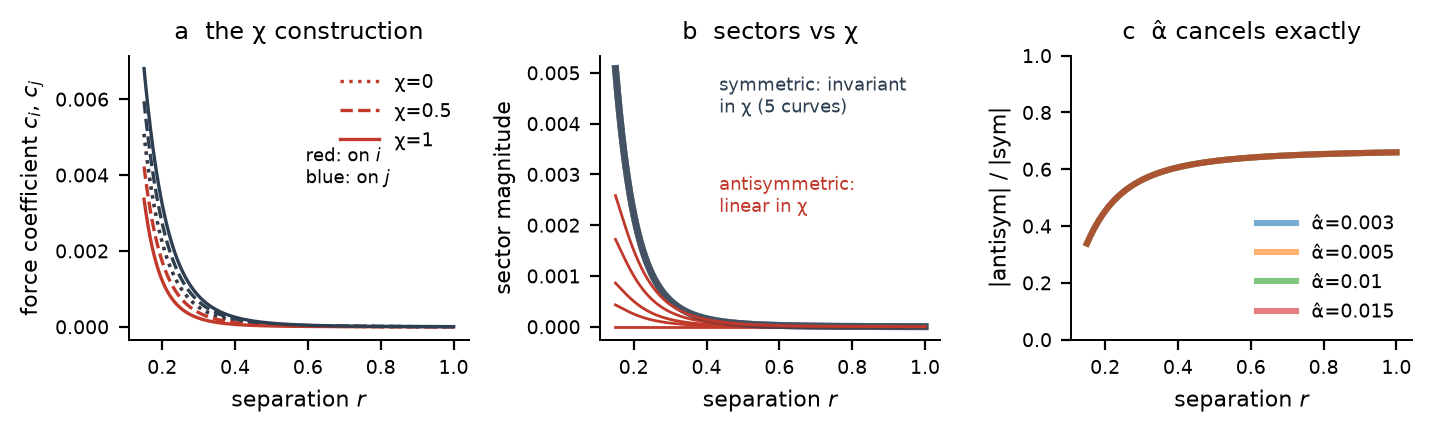
\includegraphics[width=\linewidth]{fig1_construction.png}
\caption{\textbf{The $\chi$ construction and its validation.} (a) Force coefficients $c_i$ (red) and $c_j$ (blue) against pair separation at $\chi=0,\,0.5,\,1$. At $\chi=0$ the two coincide, restoring Newton's third law exactly. (b) The symmetric sector (blue, five superposed curves at $\chi=0,\,0.25,\,0.5,\,1,\,1.5$) is invariant in $\chi$, while the antisymmetric sector (red) is exactly linear in it. (c) The antisymmetric-to-symmetric ratio for four values of the coupling strength $\hat\alpha$; the curves are indistinguishable, showing that $\hat\alpha$ cancels identically from the ratio and therefore cannot serve as a reciprocity knob.}
\label{fig:construction}
\end{figure}

Write g(r; l) $\equiv$ $\alpha$ $l^{4}$/($r^{2}$+$l^{2}$$)^{5/2}$ for the electrohydrodynamic kernel, and define the coefficients acting \emph{on} each particle,

\begin{equation}
a_i\equiv g(r;l_j),\qquad a_j\equiv g(r;l_i)
\end{equation}

\textbf{The index convention matters and is the whole content of the model:} the coefficient acting on a particle is set by the \emph{other} particle's EHD radius, so $a_{i}$ carries $l_{j}$ and $a_{j}$ carries $l_{i}$. In this notation the published law of ref. \cite{r1} reads $F_{i}$ = $-$$a_{i}$ $\mathbf{r}_{ij}$, $F_{j}$ = +$a_{j}$ $\mathbf{r}_{ij}$, and the imbalance $a_{i}$ $\neq$ $a_{j}$ is the nonreciprocity. With $\bar{g}$ $\equiv$ ($a_{i}$+$a_{j}$)/2 we replace those coefficients by

\begin{equation}
\begin{aligned}
c_i&=(1-\chi)\bar g+\chi a_i, &\qquad c_j&=(1-\chi)\bar g+\chi a_j,\\
\mathbf{F}_i&=-c_i\,\mathbf{r}_{ij}, &\qquad \mathbf{F}_j&=+c_j\,\mathbf{r}_{ij}.
\end{aligned}
\end{equation}

so that the \textbf{symmetric part ($c_{i}$+$c_{j}$)/2 = $\bar{g}$ is independent of $\chi$}, while the antisymmetric part ($c_{j}$$-$$c_{i}$)/2 = $\chi$($a_{j}$$-$$a_{i}$)/2 is exactly linear in $\chi$. At $\chi$=1, $c_{i}$ = $a_{i}$ and the law of ref. \cite{r1} is recovered exactly; at $\chi$=0, $c_{i}$ = $c_{j}$ = $\bar{g}$ and Newton's third law holds identically. In the kernel (\texttt{simulate.py}) these coefficients appear as \texttt{gi} and \texttt{gj}, with \texttt{gi} built from \texttt{l4[j]}; the same convention is used in \texttt{fdt.py}, \texttt{onsager.py} and \texttt{simulate\_rect.py}.

Validation against the compiled kernel (\texttt{tests/test\_reciprocity.py}): an isolated noise-free pair shows centre-of-mass drift 0.000$\times$10$^{0}$ at $\chi$=0, 3.95$\times$10$^{-2}$ at $\chi$=1, and exactly half that at $\chi$=0.5 (1.975$\times$10$^{-2}$, linear in $\chi$ to four digits); an equal-radius pair follows identical trajectories at $\chi$=0 and $\chi$=1 to 10$^{-14}$. Against the pre-$\chi$ code at $\chi$=1, trajectories are bitwise identical for 1000 steps, diverging only to 9.8$\times$10$^{-15}$ by 5000 steps (floating-point rounding amplified by chaos).

\subsection{$\chi$=0 gives equilibrium-compatible dynamics}

At $\chi$=0 all forces are central, pairwise and equal-and-opposite, hence conservative; mobility $\mu_{i}$ = 1/$s_{i}$ with noise variance $\sigma ^{2}$/$s_{i}$ gives $D_{i}$/$\mu_{i}$ = $\sigma ^{2}$/2, uniform across particles. Fluctuation--dissipation therefore holds, detailed balance holds for the $\chi$ = 0 \emph{equations of motion}, and the stationary probability current vanishes.

A distinction must be maintained throughout, because we later show that it matters. The $\chi$ = 0 \emph{dynamics} are equilibrium-compatible and possess a Boltzmann stationary distribution. The $\chi$ = 0 \emph{configurations realised in finite-duration simulations} are kinetically trapped and demonstrably do not sample that distribution (Section 3.5). We use ``equilibrium-compatible reciprocal dynamics'' for the former and ``kinetically trapped finite-time ensemble'' for the latter, and reserve ``equilibrium'' for the formal long-time distribution. The value of $\chi$ = 0 as a reference lies in the first sense: it guarantees that any measured current at $\chi$ $>$ 0 is attributable to the antisymmetric coupling and not to the reference itself. This is a stronger reference than the monodisperse comparison used previously, which differs from the bidisperse system in reciprocity \emph{and} polydispersity simultaneously.

\subsection{Observables}

Contact graph: edge if r $<$ 1.1($s_{i}$+$s_{j}$), minimum image. Per snapshot we compute Newman modularity $Q$ \cite{r3} of the Louvain partition, modularity of a degree-preserving (double-edge-swap) null, the number of connected components with $\ge$2 particles ($n_{\rm cl}$), and the largest-cluster fraction (lcf). Per consecutive pair we compute the adjusted Rand index between partitions (reported alongside a same-graph two-seed noise floor), the Jaccard distance between contact edge sets, and $\sigma^2_v$.

Two further observables were introduced during this work:

\textbf{Circulation.} The signed area rate in a plane of two observables, A = $1/2 \langle$x $\dot{y}$ $-$ y $\dot{x} \rangle$. At stationarity, detailed balance implies A = 0 for \emph{every} observable pair, so a nonzero value is sufficient evidence that time-reversal symmetry is broken. \textbf{The converse does not hold}: A = 0 does not establish detailed balance, because an irreversible current may simply be absent from the chosen two-dimensional projection. That asymmetry is not a technicality here --- it is precisely what Sections 3.4 and 3.11 report, and the reason the paper's negative circulation results are statements about projections rather than about the dynamics.

\textbf{Dissipation.} The kernel accumulates the Stratonovich heat delivered to the medium,

\begin{equation}
\dot Q=\sum_i \mathbf{F}_i\circ\dot{\mathbf{x}}_i,
\end{equation}

by midpoint rule \cite{r5,r26}. The dynamics are overdamped with a uniform fluctuation--dissipation ratio $D_{i}$/$\mu_{i}$ = $\sigma ^{2}$/2 $\equiv$ $T$ for every particle (Section 2.1), so the medium entropy-production rate is $\dot S_{\rm med}$ = $\dot{Q}$/T. We report the per-particle rate $\dot{Q}$/($T$ $N$); with entropy measured in units of $k_B$ this has dimensions of inverse time, per unit $\hat{t}$ in the nondimensional units of Section 2.1. Under detailed balance $\langle \dot{Q} \rangle$ = 0 identically, which is what makes this a current --- unlike edge turnover or $\sigma^2_v$, both of which are nonzero at $\chi$ = 0.

Two caveats attach to the name. The estimator is unusable at the production timestep: it subtracts two nearly cancelling terms of order $\mu |$F$| ^{2}$, and the discretisation residual dominates. It is therefore measured at dt = 6.25$\times$10$^{-4}$, restarting from equilibrated configurations. And what we report is a \emph{difference}: each configuration is probed at its own $\chi$ and again at $\chi$ = 0 with the same noise stream, and the $\chi$ = 0 value subtracted. That removes the configuration-dependent discretisation residual, which is driven by the symmetric forces and is common to both probes. This is an effective numerical control, not a derivation --- it is not equivalent to evaluating the full path-probability ratio, and it presumes the residual is $\chi$-independent at fixed configuration. We therefore speak of the \textbf{excess dissipation over the reciprocal control}, and use ``entropy production'' only where the distinction does not bear on the argument.

\subsection{Simulation campaign}

\textbf{113 simulation runs, extended by 25 continuation runs, for 138 trajectory files in total}, at five system sizes. Runs at different $\chi$ are \emph{not} statistically independent: seeds are blocked, so seed \emph{k} gives the same initial configuration and noise stream at every $\chi$. This is a common-random-number design chosen to reduce the variance of $\chi$ contrasts, and it is why we quote effect sizes rather than p-values in Section 3.2. Continuations extend existing runs and are not replicates.

\begin{table}[htbp]
\caption{The simulation campaign.}
\label{tab:1}
\begin{ruledtabular}
\begin{tabular}{p{4.96cm}p{2.16cm}p{2.58cm}p{2.51cm}p{1.15cm}}
\raggedright
series & N & box & $\hat{t}$ & runs \\
\hline
Pilot (baseline, $\hat{\alpha}$ sweep, size-ratio sweep, $\chi$ sweep) & 1,000 & L = 12 & 1$\times$10$^{5}$ & 61 \\
Paper scale ($\chi$ sweep 6 $\times$ 3, monodisperse reference $\times$ 3) & 4,000 & L = 24 & 4$\times$10$^{5}$ & 21 \\
Box scaling at fixed density 6.944 particles/area & 9,000 / 16,000 & L = 36 / 48 & 4$\times$10$^{5}$ & 6 \\
Density series at fixed $N$, $\chi$ = 1.5 & 4,000 & L = 30 / 38 / 48 & 8$\times$10$^{5}$ & 6 \\
High-drive series, $\chi$ $\in$ \{2, 3, 5, 8\} & 4,000 & L = 24 & 8$\times$10$^{5}$ & 12 \\
Rectangular-box control, aspect 1.8 : 1 & 4,000 & 32.20 $\times$ 17.89 & 8$\times$10$^{5}$ & 3 \\
Replicate at the source specification, 22.7\% type-I & 22,000 & L = 53.67 & 3.6$\times$10$^{5}$ & 4 \\
\end{tabular}
\end{ruledtabular}
\end{table}

Continuation runs extend selected conditions to $\hat{t}$ = 8$\times$10$^{5}$, and the replicate to 7.2$\times$10$^{5}$ or 1.08$\times$10$^{6}$. Paper-scale runs store 200 snapshots. Analyses use the late half of each run.

Tier-membership measurements (Section 3.10) add: entropy production probes at dt = 6.25e-4 from equilibrated configurations, with a paired same-configuration control; Onsager cross-coefficients from 40 configurations equilibrated at the operating point (chi, chi2) = (0.5, 0.5), measured by central differences with common random numbers at four window lengths; and effective-temperature measurements from 200 starts per condition, with mobility from the drift under a small force on one species and the conjugate fluctuation from the collective coordinate of that species.

The comparisons of Section 3.11 add 184 \emph{Chlamydomonas} axonemes at 1000 frames per second across eight ATP concentrations, 272,974 frames, from ref. \cite{r6}, and a separate Vicsek flock simulation (Section 2.6) run in four variants at six seeds each. Section 3.12 uses four published pairwise sociomatrices and one published behavioural table, and adds no simulation.

\textbf{Convergence.} Equilibration time grows steeply with system size, and an underequilibrated large box systematically \emph{understates} the largest cluster --- mimicking a finite characteristic cluster size. Every continuation run raised the largest-cluster fraction: +3.4\% (N=4000, $\chi$=1.5), +8.8\% (N=9000, $\chi$=1.5), +50.9\% (N=16000, $\chi$=1.5), +86.8\% (N=9000, $\chi$=1), and +68\% on average at N=22,000 (four seeds, range +24\% to +115\%). No scale-selection claim below rests on a run that has not been continued and shown to plateau. Collapse of the within-run and between-seed scatter is a more reliable convergence indicator here than a slope fit, because cluster counts fluctuate by up to 30\% within a run. That collapse is clean at N=4,000 and N=9,000 (between-seed spread in lcf falling to $\pm$0.001 at N=9,000) but not at N=16,000, where two converged seeds still differ (0.709 and 0.857); the N=16,000 point in Section 3.8 therefore carries a correspondingly wide error, which its role in the scaling fit must be read against.

\subsection{The comparison systems}

Three systems outside the colloid model are used as controls and comparisons. Because the point of each is that the \emph{same} estimator is applied, we specify the shared pipeline once.

\textbf{The circulation estimator.} For any two observables (a, b) sampled at uniform intervals, the signed area rate is A = $1/2 \langle$a $\dot{b}$ $-$ b $\dot{a} \rangle$, computed from successive differences. At stationarity, detailed balance implies A = 0 for any observable pair, so a nonzero A is sufficient evidence of broken time-reversal symmetry; a zero A is not evidence of detailed balance, since the current may lie outside the projection (Section 2.4). Significance is assessed against 80 phase-randomised surrogates per object, which preserve the power spectrum of each channel while destroying cross-channel phase relations, and reported as
$|$z$|$ = $|$A $-$ $\langle$$A_{\rm surr}$$\rangle |$ / sd($A_{\rm surr}$). We take absolute values because the sign of a principal component is arbitrary, so signed z-scores are not comparable across objects.

\textbf{Cilia.} Axoneme centrelines from ref. \cite{r6} are converted to a tangent-angle representation $\psi$(s, t) along the arclength s, which removes rigid translation. Rigid \emph{rotation} is removed by subtracting the per-frame mean angle, $\psi$ $\rightarrow$ $\psi$ $-$ $\langle\psi\rangle_s$; omitting this step leaves the whole-axoneme rotation in the signal and yields beat frequencies an order of magnitude below the known 20--50 Hz, which is how we detected the omission. The de-rotated $\psi$ is reduced by singular value decomposition to its two dominant shape modes, and the estimator is applied in that plane.

\textbf{Single colloidal clusters.} To match the level of description, individual clusters are tracked over a 101-snapshot window and represented by a low-order shape descriptor: the deviatoric part of the gyration tensor together with the normalised third and fourth mass multipoles. This is the closest available analogue of a tangent-angle representation for an object with no centreline. The descriptor is reduced by principal component analysis to two modes and the identical estimator and surrogate protocol applied. Only clusters persisting for the full window are used, which limits the comparison to three to six clusters per condition.

\textbf{Vicsek flocks.} A standard Vicsek model is run with $N$ = 800 in a periodic box $L$ = 20, interaction radius r = 1, speed v = 0.3, dt = 1, angular noise amplitude $\eta$ = 0.25, for 6000 steps of which the first 2000 are discarded:

\begin{equation}
\theta_i(t+dt)=\arg\big\langle e^{i\theta_j}\big\rangle_{j\in\mathcal{N}_i}+\omega\,dt+\eta\,U(-\pi,\pi)
\end{equation}

Four variants are used: reciprocal with the full 2$\pi$ interaction neighbourhood ($\omega$ = 0); nonreciprocal via a vision cone of half-angle 1.2 rad, so that \emph{i} may align to \emph{j} while \emph{j} does not see \emph{i}; reciprocal with an intrinsic turning rate $\omega$ = 0.02 (chiral); and chiral with a vision cone. Six seeds per variant. The coarse observable is the mean heading vector, whose two components form the plane in which the estimator is applied --- matched in spirit to the two shape modes used for the axoneme --- and polar order $| \langle$$e^{i\theta}$$\rangle |$ is reported alongside. Turning rates $\omega$ $\in$ \{0.005, 0.01, 0.02, 0.04\} are additionally used to test whether the measured area rate tracks the imposed rate.

\textbf{Dominance networks.} For a group of n individuals the net directed interaction flow $f_{\rm ij}$ = $-$$f_{\rm ji}$ is an antisymmetric edge function on the complete graph. Filling all triangles leaves no harmonic component, so the discrete Hodge decomposition is exact and two-part: f = grad(s) + curl, with the gradient part derivable from a scalar rank potential s (obtained as s = $-$$\langle f\rangle_{\rm row}$) and the curl part genuinely non-gradient. We report the cyclic fraction $\|$curl$\|$/$\|$f$\|$. The decomposition is applied to \textbf{log-odds}, not to raw net counts: a Bradley--Terry hierarchy has logit($p_{\rm ij}$) = $r_{i}$ $-$ $r_{j}$ exactly, so its log-odds flow is exactly a gradient, whereas the net-count flow is a logistic function of the rank difference and a linear decomposition of counts therefore retains a residual cyclic fraction that does not vanish with more data (Section 3.12).

Implementation details, since they affect the numbers. Win probabilities are formed with a Jeffreys-type additive smoothing, $p_{\rm ij}$ = ($w_{\rm ij}$ + $1/2$)/($w_{\rm ij}$ + $w_{\rm ji}$ + 1), which keeps the log-odds finite when a dyad is a clean sweep; dyads with no recorded interactions are set to zero flow and so contribute nothing to either component. The potential is the least-squares solution s = $-$$\langle f\rangle_{\rm row}$ with gauge $\sum$s = 0, and the norm is the unweighted Frobenius norm on the edge flow, so each dyad counts equally regardless of how many interactions it carries. Matched floors are computed from 200 regenerated Bradley--Terry replicates at the observed per-dyad counts. All four published matrices are complete comparison graphs. Rank uncertainty is not propagated into the floor, which is a limitation of the reported z-scores.

\section{Results}

\subsection{Two previously proposed knobs do not vary reciprocity}

The coupling-strength parameter $\hat{\alpha}$ \textbf{cancels exactly} from the antisymmetric/symmetric ratio
$|$$a_{i}$$-$$a_{j}$$|$/$|$$a_{i}$+$a_{j}$$|$ (notation of Section 2.2): both sectors scale linearly in it. Numerically the ratio is identical to six decimal places across $\hat{\alpha}$ $\in$ \{0.003, 0.005, 0.010, 0.015\} at every separation tested. Sweeping $\hat{\alpha}$ produced edge turnover \emph{falling} from 0.601 to 0.282 --- opposite to the prediction it was meant to test --- because $\hat{\alpha}$ raises overall attraction and condenses the system ($n_{\rm cl}$ 40 $\rightarrow$ 9).

The steric size-ratio sweep also fails, because the protocol of ref. \cite{r1} pins the EHD radii while varying steric radii; it therefore varies packing, not reciprocity. Turnover falls 506$\times$ toward the tail-large regime, but by total condensation into a single cluster ($n_{\rm cl}$ = 1.0, lcf = 1.00), not by graded suppression of fission.

This is a caution specific to simulation: in experiment a particle's EHD and steric radii are the same physical size, so the experimental size ratio does tune nonreciprocity.

\subsection{Nonreciprocity produces the fragmented morphology termed arrested coarsening}
\begin{figure}[htbp]
\centering
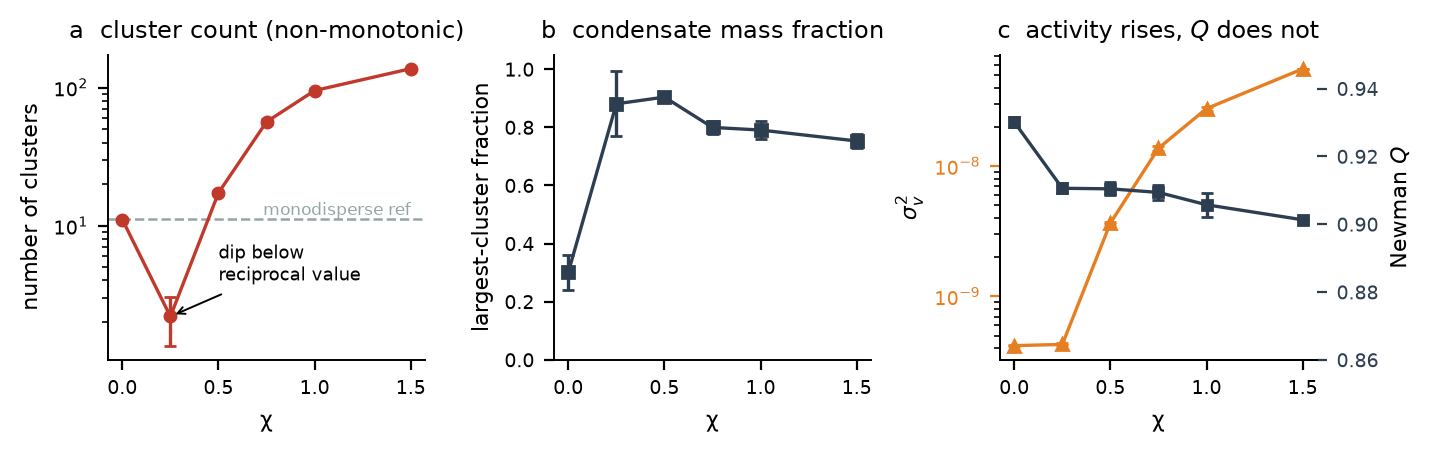
\includegraphics[width=\linewidth]{fig2_structure.png}
\caption{\textbf{Structure against $\chi$ at paper scale ($N=4000$, three seeds).} (a) Cluster count, log axis, showing the non-monotonic dip at $\chi=0.25$ to a value five times \emph{below} the reciprocal case before rising by two orders of magnitude; the dashed line is the monodisperse reference. (b) Largest-cluster fraction. (c) Activity $\sigma^2_v$ (orange, log axis) against Newman modularity $Q$ (blue, right axis) on a scale spanning only $0.86$--$0.95$: the currents rise by two orders of magnitude while $Q$ barely moves. Error bars are the standard error over seeds.}
\label{fig:structure}
\end{figure}

Paper scale, 3 seeds per level, all other parameters fixed:

\begin{table}[htbp]
\caption{Structural observables against $\chi$ at paper scale ($N=4000$, three seeds), with the monodisperse reference for comparison.}
\label{tab:2}
\begin{ruledtabular}
\begin{tabular}{lrrrrrrr}
$\chi$ & 0 & 0.25 & 0.5 & 0.75 & 1.0 & 1.5 & mono ref \\
\hline
$n_{\rm cl}$ & 11.1 & 2.2 & 17.3 & 56.5 & 95.2 & 137.3 & 11.2 \\
lcf & 0.301 & 0.881 & 0.904 & 0.800 & 0.791 & 0.753 & 0.261 \\
Q & 0.930 & 0.911 & 0.910 & 0.909 & 0.906 & 0.901 & 0.936 \\
$\sigma^2_v$ & 4.19e-10 & 4.28e-10 & 3.65e-09 & 1.37e-08 & 2.76e-08 & 5.57e-08 & 3.07e-10 \\
\end{tabular}
\end{ruledtabular}
\end{table}

Trend tests across $\chi$ (18 runs): $n_{\rm cl}$ $\rho$=+0.931 (p=2.1$\times$10$^{-8}$); $\sigma^2_v$ $\rho$=+0.975 (p=7.1$\times$10$^{-12}$). $\chi$ = 0 $\rightarrow$ 1.5: $n_{\rm cl}$ 11.1 $\pm$ 0.5 $\rightarrow$ 137.3 $\pm$ 0.5 (a factor of 12.4); $\sigma^2_v$ $\times$ 133. We quote effect sizes with seed-level scatter rather than p-values here: with three blocked seeds per level, and within-run fluctuations of up to 30\% (Section 2.5), formal significance tests on run-level means produce implausibly small p-values that reflect the variance-reduction of the blocked design rather than the evidence. The effects are large enough not to need them. Both contrasts \emph{strengthen} at paper scale relative to pilot scale, where the same ratios are 9.8$\times$ and 54$\times$, indicating the pilot runs had not reached steady state.

A word on what ``arrested coarsening'' denotes here, since Sections 3.5 and 3.8 will appear to contradict this heading. What nonreciprocity produces is the \emph{finite-time fragmented morphology} conventionally given that name: many clusters coexisting and continuously reorganising, on the timescale at which the system is observed. It does so while simultaneously \emph{unjamming} the reciprocal gel and \textbf{accelerating} growth of the largest phase (Sections 3.5 and 4.5), and the fragmented state is a long-lived transient rather than an asymptotic one (Section 3.8). The reciprocal case, not the nonreciprocal one, is the genuinely arrested state. Both statements are true and they refer to different observables --- the fragment population and the majority phase.

\textbf{The antisymmetric sector therefore alters equal-time structure.} A word on terminology, which matters because the paper also establishes kinetic trapping and long-lived transience. We use \emph{equal-time structure} for the observable class ($n_{\rm cl}$, lcf --- quantities computed from a single snapshot), \emph{late-time morphology} for what a finite-duration simulation actually realises, and \emph{stationary distribution} only for a genuine stationary ensemble, which at $\chi$ $>$ 0 we do not claim to have sampled. The result here is about the first: $n_{\rm cl}$ and lcf are single-snapshot observables; they move by an order of magnitude under a change confined to the antisymmetric coupling. The premise that a solenoidal coupling cannot alter the stationary density holds only when $\nabla \cdot$($\rho_{\rm eq}$ $\mathbf{v}$) = 0, which generic nonreciprocal couplings do not satisfy. Our measurement is of equal-time structure at late times rather than of a verified stationary density, but that is the weaker requirement: a coupling that leaves the stationary density invariant cannot move an equal-time observable at late times either.

\subsection{Newman modularity is degenerate on these networks}

Across the 14 pilot-scale conditions, cluster count spans 40$\times$ (1 $\rightarrow$ 40) while $Q$ spans 15\%, and the two are uncorrelated: Spearman $\rho$ = +0.31, p = 0.28. A 3-cluster state (Q=0.869) and a 33-cluster state (Q=0.854) are indistinguishable. Louvain's resolution limit merges communities below $\sim \sqrt{2E}$ $\approx$ 60 nodes \cite{r4}, and the degeneracy survives a 4$\times$ increase in system size. This is a known hazard of modularity maximisation rather than a peculiarity of our graphs: the modularity landscape is characteristically degenerate, with many structurally distinct partitions at near-identical $Q$ \cite{r23}, which is among the reasons inferential rather than descriptive community detection is now preferred \cite{r24}.

Modularity excess over the degree-preserving null \textbf{decreases monotonically with nonreciprocity} (0.440 at $\chi$=0 $\rightarrow$ 0.383 at $\chi$=1.5) and is \emph{highest} in the monodisperse equilibrium reference (0.462). The prediction that motivated this measurement --- that constrained organisation shows itself as a sustained modularity \emph{excess} over a null rather than as high absolute modularity \cite{r30} --- is therefore not merely unsupported when carried over to nonreciprocal coupling; the ordering is inverted.

\subsection{No circulation in coarse observables, but genuine microscopic irreversibility}

The signed area rate was measured in four observable planes at every $\chi$, at both system sizes. Every value is consistent with zero and none is distinguishable from the $\chi$=0 equilibrium null (all p $\ge$ 0.38 at paper scale, where nsnap=200 doubles the statistics).

The excess dissipation over the reciprocal control, by contrast, is clearly positive. The paired Stratonovich-heat estimator of Section 2.4 resolves it for $\chi$ $\gtrsim$ 0.75. Paired-bias-subtracted, per particle:

\begin{table}[htbp]
\caption{Excess dissipation per particle against $\chi$, paired-bias-subtracted, at pilot scale.}
\label{tab:3}
\begin{ruledtabular}
\begin{tabular}{lrrrrr}
$\chi$ ($N$ = 1000, pilot scale) & 0.25 & 0.5 & 0.75 & 1.0 & 1.5 \\
\hline
net excess dissipation & $-$5.8e-5 & $-$2.2e-5 & +8.0e-4 & +2.0e-3 & +6.5e-3 \\
\end{tabular}
\end{ruledtabular}
\end{table}

resolved for $\chi$ $\gtrsim$ 0.75 and buried in bias noise below. Fitted as a bare power law over the three levels at which it resolves ($\chi$ = 0.75, 1.0, 1.5) the sweep gives $\chi^{3.01}$, but that exponent is an artefact of fitting a single power to a two-term form; Section 3.10 resolves it. Holding the configuration fixed and varying $\chi$ over a window too short to relax gives net EPR/$\chi ^{2}$ flat to \textbf{1.27$\times$ and 1.61$\times$} on two of three configurations, confirming the expected quadratic law; the third configuration's bias probe (a single stochastic realisation) came in 2$\times$ high and is instrument noise.

\textbf{The dynamics are genuinely irreversible, and that irreversibility does not appear as circulation in any network observable measured.} Dissipation is the standard measure of how far an active system sits from equilibrium \cite{r19,r20}; the point here is that a positive value of it does not guarantee a signature in any given coarse observable.

\subsection{The reciprocal reference is a kinetically arrested gel}

At $\chi$=0 the system plateaus at lcf = 0.30 from t$\approx$1.6$\times$10$^{5}$ onward --- it does not phase separate. Three lines of evidence identify this as kinetic arrest rather than equilibrium:

\begin{enumerate}
\item Integrating the symmetric pair force gives well depths of $-$7.0 $k_BT$ (L-L), $-$6.8 $k_BT$ (L-S), $-$4.8 $k_BT$ (S-S) against $k_BT_{\rm eff}$ = $\sigma ^{2}$/2. Bonds essentially never break thermally.
\item Cluster diffusion scales as D$_{1}$/n: a 1000-particle cluster moves 0.18 in a box of 24 over an entire run. Coalescence stalls.
\item \textbf{Decisive:} the condensed configuration evolved at $\chi$=0 with no activity remains condensed (lcf 0.910 $\rightarrow$ 0.910; per-seed trajectories 0.763$\rightarrow$0.763, 1.000$\rightarrow$1.000, 0.966$\rightarrow$0.967). The condensate is equilibrium-accessible; $\chi$=0 simply cannot reach it. The same dispersed configuration is frozen at $\chi$=0 ($n_{\rm cl}$ 10.3$\rightarrow$10.0) but coarsens at $\chi$=0.25 (10.3$\rightarrow$8.7).
\end{enumerate}

Weak nonreciprocity unjams this. At matched cluster size (40--120 particles) active clusters move \textbf{10.7$\times$ faster} than thermal ones. This is an amplitude effect rather than a change of scaling, and the evidence for that is the coherence rather than the drift. The pair propulsions add incoherently at every size: the coherence $C$ $\equiv$ $| \sum$$\mathbf{p}$$|$/$\sum |$$\mathbf{p}$$|$ falls as $N^{-0.53}$ across the full range of cluster sizes observed, and C$\cdot \sqrt{N}$ varies only between 1.7 and 2.7 from $N$ $\approx$ 5 to $N$ $\approx$ 80. The net drive therefore grows as $\sqrt{N}$ and the drift speed should fall as $N^{-1/2}$ --- the same exponent as thermal diffusion, so activity cannot select a size by outrunning diffusion at one. The measured drift exponent is consistent with that over the full size range ($-$0.38 per cluster, $-$0.47 on binned means) but is not resolved over the small-to-medium range alone ($-$0.09 to $-$0.12), where the dynamic range in $N$ is too small to fit an exponent. We therefore rest the claim on the coherence measurement, which is direct, and not on the drift fit.

Consequently cluster count is \textbf{non-monotonic}: $n_{\rm cl}$ dips to 2.2 at $\chi$=0.25 (below the reciprocal 11.1) as weak activity completes the arrested phase separation, then rises to 137 as strong activity drives fission. Fluctuations peak in this crossover region (sd/mean of $n_{\rm cl}$: 7.2\% at $\chi$=0, 29.7\% at $\chi$=0.25, 18.6\% at $\chi$=0.5, 7.1\% at $\chi$=1.5).

\subsection{Attributing the reciprocal/nonreciprocal difference}

The monodisperse-versus-bidisperse comparison confounds reciprocity with polydispersity. The $\chi$=0 control separates them (paper scale):

\begin{table}[htbp]
\caption{Attribution of the monodisperse-to-bidisperse difference between polydispersity and reciprocity, at paper scale.}
\label{tab:4}
\begin{ruledtabular}
\begin{tabular}{lrrrr}
observable & mono & $\chi$=0 & $\chi$=1 & share attributable to reciprocity \\
\hline
edge turnover & 0.148 & 0.260 & 0.378 & \textbf{52\%} \\
$\sigma^2_v$ & 3.07e-10 & 4.19e-10 & 2.76e-08 & \textbf{99.6\%} \\
\end{tabular}
\end{ruledtabular}
\end{table}

$\sigma^2_v$ is a clean reciprocity probe; edge turnover is about half polydispersity.

\subsection{Observable reliability}

Edge Jaccard turnover fails as a dynamical probe on four counts: about 70\% of its $\chi$=1 value survives at $\chi$=0 where the current is provably zero (69\% at paper scale, 71\% at pilot scale); it correlates with morphology (Spearman $\rho$ = +0.77 at pilot scale, +0.62 at paper scale, against $n_{\rm cl}$); its lag-1 value is dominated by hard-cutoff flicker (0.274 at equilibrium, rising to 0.475 by lag 32 without plateau); and it is \textbf{non-monotonic in $\chi$ at paper scale}, peaking at $\chi$=0.75. A monotonic trend observed at pilot scale did not survive equilibration.

$\sigma^2_v$ as implemented is the variance of \emph{speed} over one snapshot interval (20,000 integration steps, during which particles move $\sim$0.6 radius); it is a mobility probe, not an instantaneous velocity variance, and is not directly comparable to Fig. 2d of ref. \cite{r1}.

\subsection{No characteristic cluster size is selected; the small-cluster state is transient}
\begin{figure}[htbp]
\centering
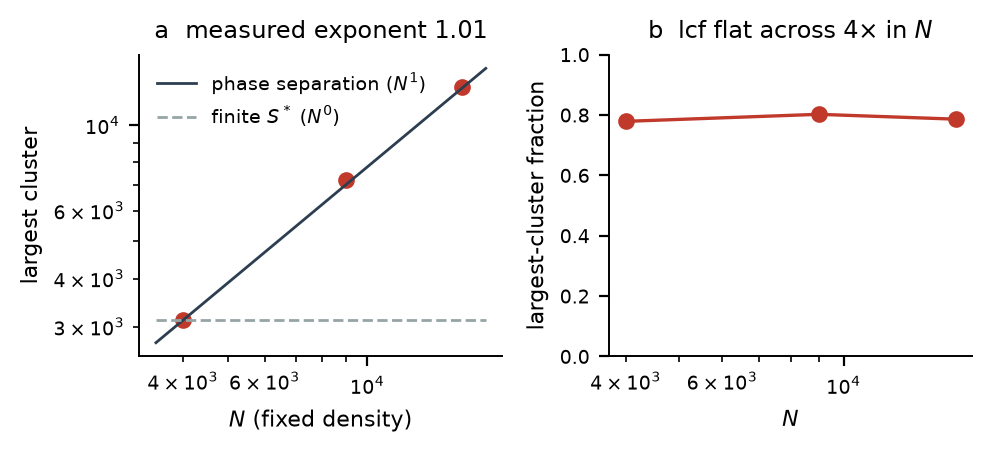
\includegraphics[width=\linewidth]{fig3_scaling.png}
\caption{\textbf{Box scaling at fixed density.} (a) Largest cluster against $N$ for three converged system sizes, with the phase-separation ($N^1$) and finite-characteristic-size ($N^0$) expectations. The measured exponent is $1.00\pm0.07$. (b) The largest-cluster fraction is flat across a fourfold range of $N$, which is the same statement without a fit.}
\label{fig:scaling}
\end{figure}

The E-vs-C tradeoff account of arrested coarsening requires the system to select a finite cluster size, which appears as an interior peak in the cluster-size distribution. Testing this requires growing the box at fixed density: a finite characteristic size $S^*$ holds the largest cluster constant (lcf $\propto$ $S^*$/N $\propto$ 1/$L^{2}$), whereas phase separation makes it grow $\propto$ $N$.

At $\chi$=1.5, densities matched exactly at 6.944 particles per unit area, all points continued to convergence:

\begin{table}[htbp]
\caption{Box scaling at fixed density $6.944$ particles per unit area, $\chi=1.5$, all points continued to a late-time plateau.}
\label{tab:5}
\begin{ruledtabular}
\begin{tabular}{rrrrrr}
N & L & largest cluster & ratio & ($N$ ratio) & lcf \\
\hline
4,000 & 24 & 3,116 & 1.00$\times$ & 1.00$\times$ & 0.779 \\
9,000 & 36 & 7,221 & 2.32$\times$ & 2.25$\times$ & 0.802 \\
16,000 & 48 & 12,581 & 4.04$\times$ & 4.00$\times$ & 0.786 \\
\end{tabular}
\end{ruledtabular}
\end{table}

\emph{A note on which lcf is which.} Largest-cluster fractions for $\chi$ = 1.5, $N$ = 4000 appear at two values in this paper and the difference is duration, not disagreement. Section 3.2's table reports 0.753, the late half of the production runs at $\hat{t}$ = 4$\times$10$^{5}$. The value here, 0.779, is the late half of the same runs continued to $\hat{t}$ = 8$\times$10$^{5}$, and is the converged one; it is also the value the rectangular-box control of Section 5 is compared against. All scale-selection claims use the continued runs.

\textbf{Largest cluster $\propto$ $N^{1.00\pm0.07}$}, where the uncertainty is the spread over all twelve combinations of one seed per system size (range 0.93 to 1.07), against 0.00 for a finite characteristic size and 1.00 for phase separation. We do not treat this as a precisely resolved exponent: it rests on three system sizes, and the two $N$ = 16,000 seeds converge to appreciably different largest-cluster fractions (0.709 and 0.857). The robust statement, which needs no fit, is that the largest-cluster fraction stays approximately constant --- mean 0.79, range 0.71 to 0.86 across all seeds and sizes --- while $N$ increases fourfold. That is inconsistent with an N-independent characteristic cluster size over the range tested, and consistent with macroscopic phase separation. The fragment population is extensive ($n_{\rm cl}$ $\propto$ $N^{0.96}$) with median cluster size 3 at every box. No interior peak appears at any size tested.

\textbf{The replicate at the source specification.} Composition was corrected to the published 5,000:17,000 (22.7\% type-I; our earlier runs used 25\%, and type-I particles carry 5.1$\times$ the EHD strength, so the excess biases toward condensation):

Four seeds, each carried forward until its largest-cluster fraction stopped drifting:

\begin{table}[htbp]
\caption{Replicate at the source specification ($N=22{,}000$, $22.7\%$ type-I): largest-cluster fraction by seed and observation window.}
\label{tab:6}
\begin{ruledtabular}
\begin{tabular}{p{1.02cm}p{4.05cm}p{2.60cm}p{3.34cm}p{2.34cm}}
\raggedright
seed & $\hat{t}$ = 0 -- 3.6$\times$10$^{5}$ (\textbf{source duration}) & 3.6 -- 7.2$\times$10$^{5}$ & 7.2$\times$10$^{5}$ -- 1.08$\times$10$^{6}$ & drift in final window \\
\hline
1 & 0.381 & \textbf{0.811} & --- & +1.1\% \\
2 & 0.479 & \textbf{0.853} & --- & +0.8\% \\
3 & 0.441 & 0.536 & \textbf{0.549} & +0.0\% \\
4 & 0.554 & 0.708 & \textbf{0.870} & $-$0.0\% \\
mean & \textbf{0.464 $\pm$ 0.037} &  & \textbf{0.771 $\pm$ 0.075} &  \\
\end{tabular}
\end{ruledtabular}
\end{table}

Seeds 3 and 4 were still drifting after the second window and were therefore extended to a third. All four then show no detectable drift over their final observation window. We distinguish that from ensemble or asymptotic convergence, which we cannot demonstrate: a within-run plateau in a system whose cluster diffusion has become extremely slow is consistent with a genuine steady state and also with arrest at a configuration-dependent macrostate. The seed heterogeneity below suggests the latter, so we describe these as late-time plateaus rather than asymptotic values. The paired increase from the source duration to the converged state is \textbf{+0.307 $\pm$ 0.070, a 66\% rise} (paired t = +4.4, p = 0.022), and every seed moves in the same direction, by between 24\% and 113\%.

Two features deserve comment. An earlier two-seed estimate gave 0.415 $\rightarrow$ 0.831; the four-seed figures are 0.464 $\rightarrow$ 0.771 with a wider spread, so the two-seed version somewhat overstated the magnitude. More interestingly, \textbf{the converged state is not unique}: three seeds settle at 0.81--0.87 while seed 3 settles at 0.549 and stays there. That heterogeneity is consistent with the kinetic-arrest picture of Section 3.5 --- a configuration that has separated into two large clusters which then cannot find each other has no route to a single condensate on any accessible timescale. The asymptotic largest-cluster fraction is therefore configuration-dependent, which is itself a statement about arrest rather than about coarsening.

Two results follow. First, \textbf{composition does not explain the discrepancy}. At convergence the 22.7\% replicate reaches lcf = 0.771 $\pm$ 0.075, squarely within the 0.78--0.79 seen across our 25\% runs at $N$ = 4,000 to 16,000, rather than the 47\% shortfall the underequilibrated comparison suggested. This is a coarse comparison rather than a controlled one --- the replicate differs from those runs in system size and in $\chi$ as well as in composition --- but it is enough to rule composition out as the explanation, since correcting it moved the converged value by a few per cent and not in the direction that would reconcile us with the source. Second, \textbf{at the source paper's own simulation duration this reimplementation reproduces its reported state} --- a majority of particles outside the largest cluster, median cluster size 3 --- and the same system continued to twice that duration phase-separates.

The small-cluster state is therefore a long-lived transient of this model rather than its steady state. This is both a validation of the reimplementation (it reaches the published state under the published conditions) and a limitation of the model (that state does not persist).

\subsection{The selected scale is an event-rate crossover, not a stable cluster size}
\begin{figure}[htbp]
\centering
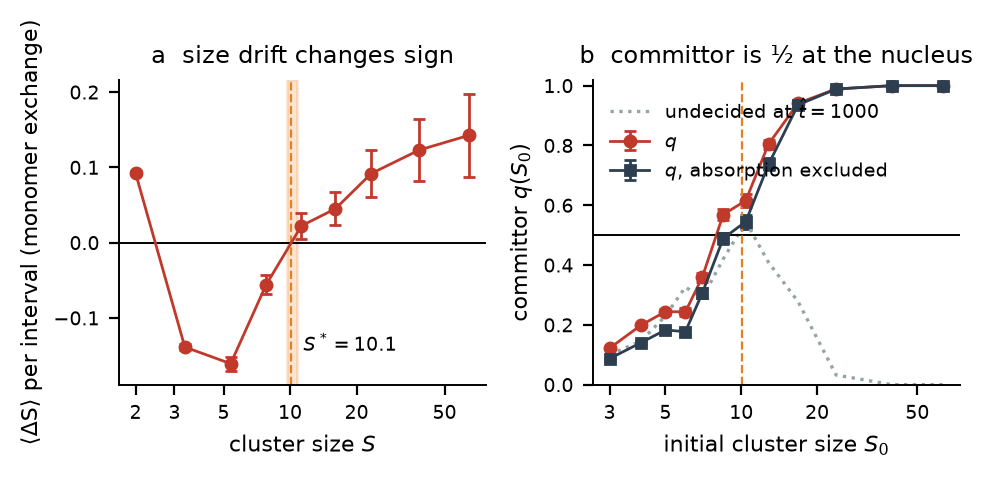
\includegraphics[width=\linewidth]{fig4_rates.png}
\caption{\textbf{The event-rate crossover.} (a) Per-cluster split and merge rates against cluster size, measured at $\Delta t=50$ from equilibrated configurations ($105{,}708$ cluster observations). The rates cross between the size-5 and size-10 bins. (b) Their difference, showing the sign change. Splitting dominates below the crossing, merging above it.}
\label{fig:rates}
\end{figure}

Two further measurements resolve what the system selects. \textbf{Fragments} --- all clusters except the largest --- have size statistics independent of system size: mean 5.02, 4.78, 5.34 particles at $N$ = 4,000, 9,000, 16,000, with an N-independent cutoff (p99 = 33, 35, 26) and a constant fragment mass fraction of $\sim$16\%. A scale is therefore selected.

Its nature follows from resolving merge and split events directly. At the production snapshot interval this is impossible --- a small cluster is typically absorbed within one interval, so tracking reports condensate size rather than a growth increment. Repeating from equilibrated configurations at $\Delta$t=50 (105,708 cluster-observations, 3 seeds) gives per-cluster rates:

\begin{table}[htbp]
\caption{Per-cluster split and merge rates against cluster size, measured at $\Delta t=50$ from equilibrated configurations.}
\label{tab:7}
\begin{ruledtabular}
\begin{tabular}{lrrrrrr}
cluster size & $\sim$2 & $\sim$5 & $\sim$10 & $\sim$19 & $\sim$45 & $\sim$74 \\
\hline
split rate & 0.333 & \textbf{0.453} & 0.254 & 0.181 & 0.081 & 0.086 \\
merge rate & 0.319 & 0.312 & \textbf{0.334} & 0.283 & 0.269 & 0.145 \\
\end{tabular}
\end{ruledtabular}
\end{table}

The rates cross between the size-5 and size-10 bins; interpolating gives \textbf{$S^*$ $\approx$ 7--8 particles}, with splitting dominant below and merging above. We do not resolve the crossing more finely than those two bins bracket it. Per-bin uncertainties were not retained by the analysis that produced this table, so the quoted 7--8 should be read as the interpolated crossing of two binned rate curves and not as a measurement with an error bar --- a gap in our own reporting, and one that the drift and committor measurements named below would close along with the interpretation. We call this an \textbf{event-rate crossover scale} rather than a critical nucleus: a crossing of per-cluster event \emph{rates} is not by itself a zero of the size drift $\langle \Delta S|S\rangle$/$\Delta$t, and a critical nucleus would properly be established by that drift changing sign, or by a committor q($S^*$) $\approx$ $1/2$. Both remain to be measured. The crossing is nonetheless the scale that separates the below-crossover population from the condensate, and the fragment population (mean $\approx$ 5) sits below it. We avoid calling that population a subcritical vapour: without the drift or committor measurement the nucleation reading is an analogy, not a result.

\textbf{The fragment scale is independent of density as well as of system size.} Holding $N$ = 4000 and $\chi$ = 1.5 fixed while expanding the box dilutes the suspension from the baseline 6.944 particles per unit area down to 1.736:

\begin{table}[htbp]
\caption{Density dependence at fixed $N=4000$ and $\chi=1.5$: the condensate is strongly density-dependent, the fragment scale much less so.}
\label{tab:8}
\begin{ruledtabular}
\begin{tabular}{lrrrr}
density & 6.944 (L=24) & 4.444 (L=30) & 2.770 (L=38) & 1.736 (L=48) \\
\hline
largest-cluster fraction & 0.779 & 0.534 & 0.130 & 0.038 \\
number of clusters & 141 & 277 & 429 & 498 \\
\textbf{mean fragment size} & \textbf{5.0} & \textbf{5.6} & \textbf{6.9} & \textbf{6.3} \\
\end{tabular}
\end{ruledtabular}
\end{table}

The condensate is strongly density-dependent and essentially gone by the lowest density: there is a threshold below which the majority phase does not form. We restrict the fragment claim to the three densities at which a condensate exists, since at $\rho$ = 1.736 there is no majority phase and ``fragments'' and ``all clusters'' are the same population --- not the regime the comparison is meant to test. Over those three the mean fragment size moves from 5.0 to 6.9, a 38\% swing across a 2.5-fold change in density. That is a good deal weaker than ``independent'', and we claim only that the fragment scale stays within a narrow band --- the same band it occupies over a fourfold change in system size (Section 3.8) --- while the condensate fraction changes by a factor of six. The lowest- density point was not continued and is the least converged of the four.

The state is thus a condensate coexisting with a population of small clusters that are, on average, more likely to split than to merge. Whether the crossing is a genuine nucleation barrier in the thermodynamic sense is exactly the question the drift and committor measurements above would settle. What is established is that no mechanism caps cluster size, consistent with \S{}3.8: the largest cluster grows as $N^{1.00\pm0.07}$ and the system phase-separates.

\subsection{The limits of three commonly used nonequilibrium diagnostics}
\begin{figure}[htbp]
\centering
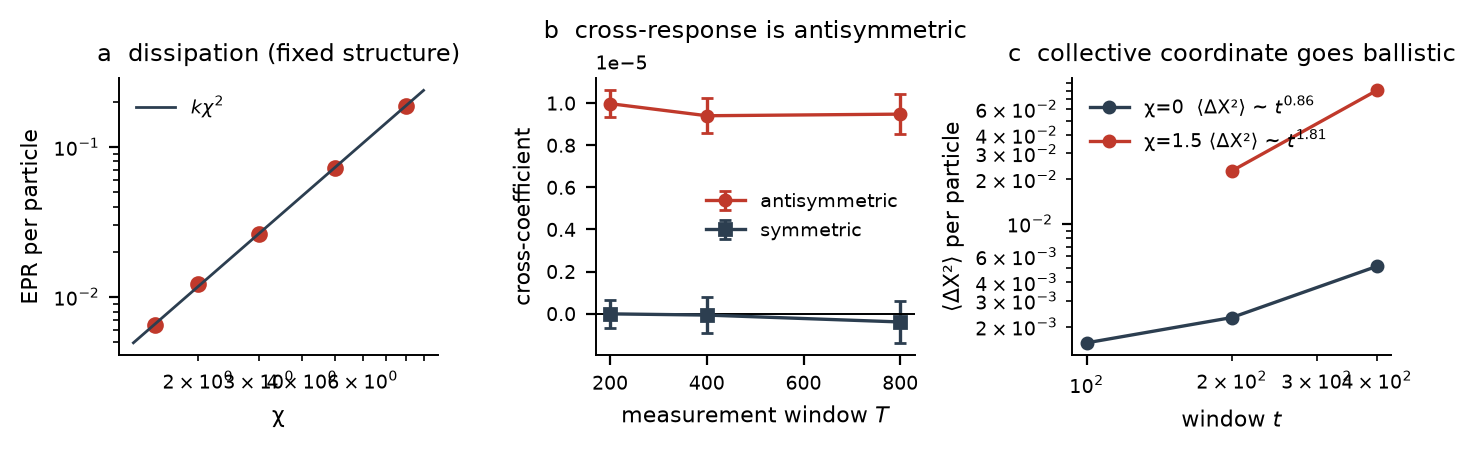
\includegraphics[width=\linewidth]{fig5_thermo.png}
\caption{\textbf{Dissipation and response.} (a) Excess dissipation per particle against $\chi$, each point probed from a configuration equilibrated at that $\chi$, with the quadratic form. (b) Symmetric and antisymmetric parts of the differential cross-response between two nonreciprocal channels, against measurement window. For channels of identical structure the symmetric part is consistent with zero at every window while the antisymmetric part is stable; the structurally dissimilar control is plotted alongside on the same axes, where the pattern inverts. (c) Effective temperature against measurement window: flat at $\chi=0$, where it calibrates to $k_BT$, and growing as $t^{0.89}$ at $\chi=1.5$ with no plateau. Inset: mean-squared displacement of the system centre of mass, near-ballistic at $\chi=1.5$ over these windows ($t^{1.96}$) and diffusive at $\chi=0$ ($t^{1.01}$).}
\label{fig:thermo}
\end{figure}

The preceding sections establish what nonreciprocity does to this system. We now ask what kind of variational description it admits. The question is easy to render vacuous --- a framework asserting that ``some variational principle applies'' forbids nothing --- so we treat tier membership as an experimental matter. We stress that the following is a working taxonomy of \emph{commonly invoked diagnostics}, not an established classification: the existence of a single effective temperature in particular is a nonequilibrium construct in the sense of Cugliandolo and Kurchan \cite{r11}, and is neither necessary nor sufficient for near-equilibrium response. With that caveat:

\begin{table}[htbp]
\caption{A working taxonomy of commonly invoked variational tiers and the experimental signatures usually associated with them.}
\label{tab:9}
\begin{ruledtabular}
\begin{tabular}{p{1.17cm}p{2.61cm}p{5.13cm}p{4.89cm}}
\raggedright
tier & regime & variational object & signature \\
\hline
I & equilibrium & free energy; MaxEnt & EPR = 0; detailed balance; Boltzmann \\
II & linear response & Rayleighian $R$ = $\dot{\Phi}$ + $\Psi$, $\Psi$ quadratic in rates \cite{r21} & fluxes linear in the forces; Onsager reciprocity among conjugate pairs \\
III & far from equilibrium & no general principle & nonlinear flux--force relations; reciprocity fails \\
\end{tabular}
\end{ruledtabular}
\end{table}

It is worth noting at the outset that least action does not fail for nonreciprocal systems in the way sometimes supposed. The Onsager--Machlup action S[x] = $\int$ ($\dot{x}$ $-$ $\mu$F)$^{2}$/4D dt is well defined for \emph{any} drift field, gradient or not. What fails is the equilibrium corollary --- that the stationary distribution is exp($- \beta$U) and that structure is selected by minimising an energy. That corollary, and not least action itself, is what the solenoidal proposal of Section 1 relied upon.

We tested three tier-II signatures.

\textbf{Quadratic dissipation.} Entropy production per particle, measured with the paired-configuration protocol of Section 2.4 and bias-subtracted against a same-configuration $\chi$ = 0 control:

\begin{table}[htbp]
\caption{Excess dissipation at high drive and its ratio to $\chi^2$.}
\label{tab:10}
\begin{ruledtabular}
\begin{tabular}{lrrrrr}
$\chi$ & 1.5 & 2 & 3 & 5 & 8 \\
\hline
EPR & 6.53e$-$3 & 1.22e$-$2 & 2.63e$-$2 & 7.25e$-$2 & 1.88e$-$1 \\
EPR/$\chi ^{2}$ & 2.90e$-$3 & 3.04e$-$3 & 2.93e$-$3 & 2.90e$-$3 & 2.93e$-$3 \\
\end{tabular}
\end{ruledtabular}
\end{table}

EPR = k$\chi ^{2}$ with k $\approx$ 2.93 $\times$ 10$^{-3}$, flat to \textbf{4.8\%} across the four points at $\chi$ = 2 to 8 --- a fourfold range of drive and a fifteenfold range of entropy production --- and to the same 4.8\% when the $\chi$ = 1.5 point is included. Those four points are at $N$ = 4000 and the $\chi$ = 1.5 point at $N$ = 1000, which is why we quote the range over the former.

We are careful about what this does and does not test, and two things have to be separated.

\emph{This row is not a fixed-configuration measurement.} Each $\chi$ is probed from a configuration equilibrated at that same $\chi$, so structure co-varies with drive along the row. That makes the clean quadratic less trivial than a frozen-structure result would be, but also harder to attribute, since two things change together.

\emph{At genuinely frozen configuration the quadratic form is largely fixed by construction.} The antisymmetric force is exactly linear in $\chi$; the dynamics are overdamped with configuration-independent mobility; and the symmetric sector is conservative, so its own contribution to the Stratonovich heat is an exact differential which averages to zero in a stationary state. What remains contains a term linear in $\chi$ and a term quadratic in it, and the quadratic term must dominate at large $\chi$ whatever the system does. The only informative question is therefore whether the linear cross-term is resolvable, and Section 3.4 reports the direct test: holding a configuration fixed and varying $\chi$ over a window too short to relax gives net EPR/$\chi ^{2}$ flat to 1.27$\times$ and 1.61$\times$ on two of three configurations --- appreciably noisier than the 4.8\% above, and not a sharp enough measurement to isolate a linear term.

The measurement is therefore best read as a \textbf{validation of the entropy-production estimator} across a fifteenfold range of signal --- non-trivial given the discretisation problems documented in Section 5 --- rather than as an independent test of linear response.

\emph{The linear cross-term is resolvable, and it accounts for the apparent $\chi ^{3}$.} Fitting the two-term form that the argument above predicts, weighted by the standard error on each point:

\begin{table}[htbp]
\caption{Weighted fits of the excess dissipation to a pure quadratic and to the two-term form the construction predicts.}
\label{tab:11}
\begin{ruledtabular}
\begin{tabular}{p{3.38cm}p{4.61cm}p{6.26cm}}
\raggedright
range & pure a$\chi ^{2}$ & a$\chi ^{2}$ + b$\chi$ \\
\hline
N = 1000, $\chi$ = 0.25--1.5 & $\chi ^{2}$/dof = 8.35 & a = 3.96(34)$\times$10$^{-3}$, \textbf{b = $-$1.78(32)$\times$10$^{-3}$}, $\chi ^{2}$/dof = 1.13 \\
N = 4000, $\chi$ = 2--8 & a = 2.93(2)$\times$10$^{-3}$, $\chi ^{2}$/dof = 0.11 & b = $-$0.7(3.3)$\times$10$^{-4}$, consistent with zero \\
\end{tabular}
\end{ruledtabular}
\end{table}

At low drive a pure quadratic is a poor fit and the linear term is resolved at 5.6$\sigma$, with a \emph{negative} sign; at high drive the quadratic alone already fits and the linear term is unresolvable, as it must be once the $\chi ^{2}$ term dominates. Adding a constant offset improves neither fit significantly (c = 4.5 $\pm$ 2.5 $\times$ 10$^{-4}$ at low drive, 1.8$\sigma$), which rules out a residual additive bias in the paired subtraction as the explanation.

So the data are consistent with the two-term form the construction argument predicts, EPR = a$\chi ^{2}$ + b$\chi$ with b $<$ 0, and the $\chi^{3.01}$ of Section 3.4 is what a bare power-law fit returns in the region where the negative linear term is still being outgrown. We stop short of calling this a single form fitted across the whole range, for two reasons that a referee would raise and that we cannot fully remove. The two fits above are at different system sizes as well as different drive ranges, so $N$ is confounded with $\chi$ here; and their quadratic coefficients differ by 35\% (3.96 against 2.93 $\times$ 10$^{-3}$), by far more than the quoted errors. Over a narrow drive window a and b are strongly anticorrelated, so a larger a is precisely how a spurious negative b would be absorbed, and the 5.6$\sigma$ on b is conditional on a floating free. The defensible statement is therefore that the data require a term beyond the pure quadratic at low drive, that its sign is negative, and that its magnitude is bounded rather than sharply determined. What the result is \emph{not}, in any reading, is evidence of linear response: the quadratic term's dominance at large $\chi$ is built into the construction.

\textbf{Onsager reciprocity.} This requires a second, independent drive. A uniform field applied to one species is unsuitable: the system is isotropic, so the species drift vanishes at zero field for every $\chi$ and the cross-coefficient is zero by symmetry rather than by physics, rendering the test vacuous. We instead opened a second nonreciprocal channel in the collision force, with its own parameter $\chi _{2}$ and the same pair-co-propulsion structure as the electrohydrodynamic one. Entropy production is then bilinear in two internal thermodynamic forces,

\begin{equation}
T\,\dot S=\chi J_1+\chi_2 J_2,\qquad J_1=\sum \mathbf{f}_1\!\cdot\!\mathbf{v},\qquad J_2=\sum \mathbf{f}_2\!\cdot\!\mathbf{v},
\end{equation}

identifying ($\chi$, $\chi _{2}$) as forces and (J$_{1}$, J$_{2}$) as their conjugate fluxes. Measured at the operating point ($\chi$, $\chi _{2}$) = (0.5, 0.5) from configurations equilibrated at that point:

\begin{table}[htbp]
\caption{Differential cross-response between two nonreciprocal channels of \emph{identical} structure, at the operating point $(\chi,\chi_2)=(0.5,0.5)$.}
\label{tab:12}
\begin{ruledtabular}
\begin{tabular}{p{1.88cm}p{3.98cm}p{1.76cm}p{4.25cm}p{1.48cm}}
\raggedright
window T & symmetric part (L$_{12}$+L$_{21}$)/2 & t & antisymmetric part (L$_{12} -$L$_{21}$)/2 & t \\
\hline
200 & $-$1.08e$-$8 $\pm$ 6.5e$-$7 & $-$0.02 & +9.98e$-$6 $\pm$ 6.3e$-$7 & +15.8 \\
400 & $-$6.81e$-$8 $\pm$ 8.6e$-$7 & $-$0.08 & +9.40e$-$6 $\pm$ 8.2e$-$7 & +11.4 \\
800 & $-$3.96e$-$7 $\pm$ 9.9e$-$7 & $-$0.40 & +9.48e$-$6 $\pm$ 9.6e$-$7 & +9.9 \\
\end{tabular}
\end{ruledtabular}
\end{table}

The symmetric part of the cross-coupling vanishes at every window length, while the antisymmetric part is large and stable: \textbf{the measured differential cross-response is predominantly antisymmetric}, L$_{12}$ $\approx$ $-$L$_{21}$.

\textbf{A structurally dissimilar second channel does not reproduce this.} Because both channels above were built with the same pair-co-propulsion structure, the antisymmetry may follow from that construction symmetry rather than from any physical relation. We therefore repeated the measurement with a second channel made structurally unlike the first --- cubic rather than linear size contrast, weighted toward the outer part of the overlap rather than uniform across it --- from configurations equilibrated at the operating point with that channel:

\begin{table}[htbp]
\caption{The same measurement with a structurally \emph{dissimilar} second channel. The pattern inverts, which is why the reciprocity reading is withdrawn.}
\label{tab:13}
\begin{ruledtabular}
\begin{tabular}{rrrrr}
window T & symmetric part & t & antisymmetric part & t \\
\hline
200 & +8.67e$-$7 $\pm$ 4.3e$-$7 & +2.04 & +2.16e$-$6 $\pm$ 4.2e$-$7 & +5.2 \\
400 & +1.62e$-$6 $\pm$ 5.2e$-$7 & +3.12 & +1.17e$-$6 $\pm$ 5.1e$-$7 & +2.3 \\
800 & +2.70e$-$6 $\pm$ 5.9e$-$7 & +4.57 & \textbf{+1.18e$-$8 $\pm$ 5.9e$-$7} & \textbf{+0.0} \\
\end{tabular}
\end{ruledtabular}
\end{table}

The pattern inverts. With dissimilar channels the antisymmetric part \emph{decays to zero} while a symmetric part grows and becomes significant --- the opposite of the identical-channel case, where the antisymmetric part plateaued and the symmetric part remained at zero throughout. The result is reproduced at two equilibration lengths ($T$ = 2$\times$10$^{4}$ and 1$\times$10$^{5}$), and neither component has plateaued at the longest window, so the dissimilar case is not itself converged; but its direction is consistent and unambiguous.

\textbf{We therefore do not claim antisymmetry as a general property of the cross-response between nonreciprocal channels.} It is observed robustly when the two channels share a structure and is absent when they do not, which is what the construction-symmetry explanation predicts. The identical-channel measurement stands as a measurement; its interpretation as a physical reciprocity relation does not survive this control.

We deliberately stop short of calling either measurement Onsager--Casimir reciprocity \cite{r7,r8}. That identification would require a defined microscopic time-reversal operation with the parities of all time-odd control parameters specified, and it cannot be inferred retrospectively from an observed sign. Three further caveats apply independently of the control just described. The coefficients are measured about a nonequilibrium operating point rather than about equilibrium; $\chi$ and $\chi _{2}$ are internal coupling constants in the equations of motion, not thermodynamic affinities, so the bilinear identity above is a definition rather than a derivation; and the two-channel construction is ours, not a feature of the source model.

For completeness we record the reading these measurements were originally given, and why it was withdrawn. Entropy production is the quadratic form EPR = $\sum$ $L_{\rm ij}$ $X_{i}$ $X_{j}$, to which only the symmetric part of $L$ contributes, so a purely antisymmetric off-diagonal block dissipates nothing; an antisymmetric cross-coupling would therefore be \emph{reactive} rather than dissipative, and that would explain why the entropy production reduces to a single-coefficient quadratic. A naive parity argument predicts the opposite --- both fluxes have the form $\sum$ f $\cdot$ v with f even and v odd under time reversal, making both odd and their signatures equal --- so the observed antisymmetry appeared to demand a physical mechanism, for which the most economical candidate was a \emph{gyroscopic} coupling in the space of collective coordinates, Magnus- or Coriolis-like, entering the response matrix antisymmetrically without contributing to dissipation. The dissimilar-channel control does not support that reading. We report it here as the hypothesis the control was built to test and did not confirm, rather than as a result. \textbf{A defensible Onsager test in this model would require an equilibrium Green--Kubo derivation or an explicit Fokker--Planck computation of $L_{\rm ij}$, and we do not have one.}

\textbf{Effective temperature.} At equilibrium the fluctuation--dissipation theorem \cite{r25} fixes D/$\mu$ = $k_BT$ for every degree of freedom; here mobility is 1/$s_{i}$ and the noise variance $\sigma ^{2}$/$s_{i}$, so D/$\mu$ = $\sigma ^{2}$/2 exactly for both species. Out of equilibrium the ratio defines an effective temperature, and a single $T_{\rm eff}$ shared across degrees of freedom is a tier-II signature. We measured mobility from the drift under a small force applied to one species, and the conjugate fluctuation from the collective coordinate $X$ = $\sum_{i\in\,{\rm species}}$ $x_{i}$, with perturbed and unperturbed runs sharing a noise stream. Linear response was verified separately: $T_{\rm eff}$ is independent of the perturbation strength down to f = 3 $\times$ 10$^{-6}$.

At equilibrium the estimator behaves as it must, returning $T_{\rm eff}$/$k_BT$ = 0.94, 1.04 and 1.09 for the large species at measurement windows $T$ = 200, 400 and 800 (150 starts each) --- unity within error and window-independent to an exponent of +0.11. The small species agrees. That calibration is what makes the out-of-equilibrium result interpretable.

Out of equilibrium there is no window-independent value. At $\chi$ = 1.5 the same estimator gives \textbf{5.18 $\pm$ 0.45, 9.54 $\pm$ 0.80 and 17.66 $\pm$ 1.54} over the same three windows, growing as $t^{+0.89}$ with no sign of a plateau. The fluctuation is strongly superdiffusive ($\langle \Delta X^2\rangle$ $\sim$ $t^{1.86}$) while the response stays linear in time, so the apparent diffusion coefficient grows with the observation window.

\textbf{Part of that superdiffusion is whole-system drift.} Nonreciprocal forces do not sum to zero over the system, so there is a net internal force and the centre of mass drifts. (The dynamics are overdamped and carry no momentum as a state variable; ``net internal force'' and ``centre-of-mass drift'' are the right descriptions, not ``net momentum''.) Over the windows used for this measurement the centre of mass moves near-ballistically, $\langle \Delta R^2\rangle$ $\sim$ $t^{1.96}$ at $\chi$ = 1.5 against $t^{1.01}$ at $\chi$ = 0. Since our response is a paired difference under common random numbers, that drift cancels from the response but not from the fluctuation. Removing the centre-of-mass displacement from the fluctuation reduces the exponent from 1.86 to 1.47, so roughly half the excess growth is the aggregate translating.

\textbf{How far that drift generalises is limited, and we checked.} Two controls bound it. First, it is persistent only over short windows: across the full production runs the centre-of-mass exponent is 1.72 $\pm$ 0.11 rather than 1.96, and the drift direction between the two halves of a run has autocorrelation +0.50 on average, reversing outright in 4 of 16 runs. The motion is therefore window-limited near-ballistic crossing over toward diffusive, not persistent self-propulsion. Second, the amplitude is consistent with vanishing in the thermodynamic limit. Section 3.5 shows pair propulsions add incoherently, so the net internal force should grow as $\sqrt{N}$ and the drift speed fall as $N^{-1/2}$. Pooling sixteen runs from $N$ = 4000 to 22,000 gives d(log $V_{\rm com}$)/d(log $N$) = $-$0.42 with a bootstrap 95\% interval of [$-$0.78, $-$0.03] --- consistent with $-$1/2, and excluding N-independence only marginally. The seed scatter within a single condition reaches a factor of 2.4, comparable to the effect across the range tested, so we do not claim this is resolved. What we claim is that the drift is a \textbf{finite-size effect of the expected magnitude}, that it contaminates the effective-temperature measurement at the sizes we simulate, and that the incoherence result of Section 3.5 predicts it should weaken as $N^{-1/2}$.

\textbf{It does not, however, rescue the effective temperature, and we report the failed control explicitly.} The drift-removed variant does not survive its own equilibrium calibration: at $\chi$ = 0 it returns 0.17, 0.11 and 0.10 $k_BT$ rather than unity, because removing the drift from the fluctuation while leaving the paired response untouched breaks the conjugacy the Einstein relation requires. Its absolute values are therefore not temperatures. Measured against its own equilibrium value --- the only defensible way to use it --- the excess at $\chi$ = 1.5 is 5.9, 11.5 and 20.0, growing at $t^{+0.88}$ against $t^{+0.78}$ for the raw estimator. The growth is not an artifact of the coordinate.

\begin{table}[htbp]
\caption{Displacement scaling and effective temperature at $\chi=0$ and $\chi=1.5$, raw and with the system centre-of-mass drift removed.}
\label{tab:14}
\begin{ruledtabular}
\begin{tabular}{p{6.07cm}p{3.64cm}p{4.54cm}}
\raggedright
 & $\chi$ = 0 & $\chi$ = 1.5 \\
\hline
system centre of mass, $\langle \Delta R^2\rangle$ & $t^{1.01}$ & \textbf{$t^{1.96}$} \\
species coordinate, $\langle \Delta X^2\rangle$ & $t^{1.08}$ & $t^{1.86}$ \\
species coordinate, drift removed & $t^{0.59}$ & $t^{1.47}$ \\
$T_{\rm eff}$/$k_BT$ at $T$ = 200 / 400 / 800 & 0.94 / 1.04 / 1.09 & \textbf{5.18 / 9.54 / 17.66} \\
\end{tabular}
\end{ruledtabular}
\end{table}

A3 therefore fails, and fails for the reason originally reported: over the windows accessible to us, the fluctuation--dissipation ratio on this coordinate is not a temperature. What the controls add is a sharper diagnosis. About half the effect is the aggregate translating under a net internal force --- a finite-size, window-limited effect rather than a new phenomenon --- and the residue is internal. We would previously have called the centre-of-mass drift a clean physical result standing on its own; the N-scaling and decorrelation controls do not support that, and it is reported here as a bounded finite-size observation.

We put the negative verdict carefully. What fails is the Einstein-ratio interpretation on this coordinate. That is not the same as demonstrating a nonlinear flux--force relation, and we do not claim the stronger statement.

\emph{The species comparison, by contrast, is an artifact and should be discarded.} An earlier version of this work read the large--small difference at $\chi$ = 1.5 as evidence bearing on whether one temperature is shared across degrees of freedom. It is not: once the system drift is removed, $X_{\rm rel}$($L$) + $X_{\rm rel}$($S$) = 0 identically, so the two species coordinates are one degree of freedom up to sign, and their apparent temperatures must differ by exactly ($n_{S}$/$n_{L}$)($\mu_{S}$/$\mu_{L}$) = 6.85. The measured ratio is 6.7, and the variance ratio is 3.0000 to five figures. Testing whether a single temperature is shared would require genuinely independent coordinates, which collective species coordinates in a two-component mixture are not.

\textbf{Interpretation: no tier-II signature is established.} We set out expecting these three diagnostics to place the system in a tier. They do not, and they fail in three different ways.

The quadratic dissipation is real and cleanly measured, but weakly diagnostic. Its principal value is as a validation of the entropy-production estimator across a fifteenfold range of signal --- which is not nothing, given the discretisation problems documented in Section 5 --- rather than as independent evidence of linear response. The Onsager measurement returned a stable, plateau-tested antisymmetry that the dissimilar-channel control shows to be most parsimoniously a property of how we built the second channel; it does not survive as a physical reciprocity relation. The effective temperature is the one that returns a definite negative: it grows without bound with the observation window, calibrates correctly at equilibrium, and survives a control that removes the whole-system drift responsible for about half of the growth.

The honest summary is that \textbf{tier membership is undetermined by these measurements}. Two of the three diagnostics are defeated by their own construction rather than by the physics --- one is near-tautological given how $\chi$ is built, the other an artifact of giving two response channels the same structure --- and the third returns a negative whose interpretation is narrower than it looks: what fails is the Einstein-ratio reading on a particular coordinate, not linear response in the formal sense. An earlier version of this work read all three as placing the system in the linear-response tier. That reading did not survive the dissimilar-channel control, and we state the revised position rather than the original one.

We none the less think the exercise was worth conducting, and record its outcome in this form deliberately. A framework asserting that ``some variational principle applies'' forbids nothing; what makes tier claims falsifiable is that each tier carries experimental signatures and that membership be \emph{measured}. What this section demonstrates is that measuring it honestly is harder than the taxonomy suggests. Two of the three signatures proved near-tautological or construction-dependent once examined closely, and the third proved not to be a well-defined quantity at all. That is a result about the diagnostics as much as about the system, and it is the reason we present the taxonomy above as a working list of commonly invoked tests rather than as a classification.

One boundary should be stated explicitly in any case, because our own data mark it. Entropy production is quadratic \emph{at fixed structure}, but the structural response to $\chi$ is strongly non-linear: cluster count is non-monotonic, dipping at $\chi$ = 0.25 before rising by an order of magnitude (Section 3.5). Whatever variational description ultimately applies to this system can at best govern its dynamics at fixed structure; \emph{structure selection} is a non-equilibrium transition that no current variational principle covers. Identifying that gap seems to us more useful than obscuring it.

\subsection{A biological comparison: does irreversibility survive coarse-graining?}
\begin{figure}[htbp]
\centering
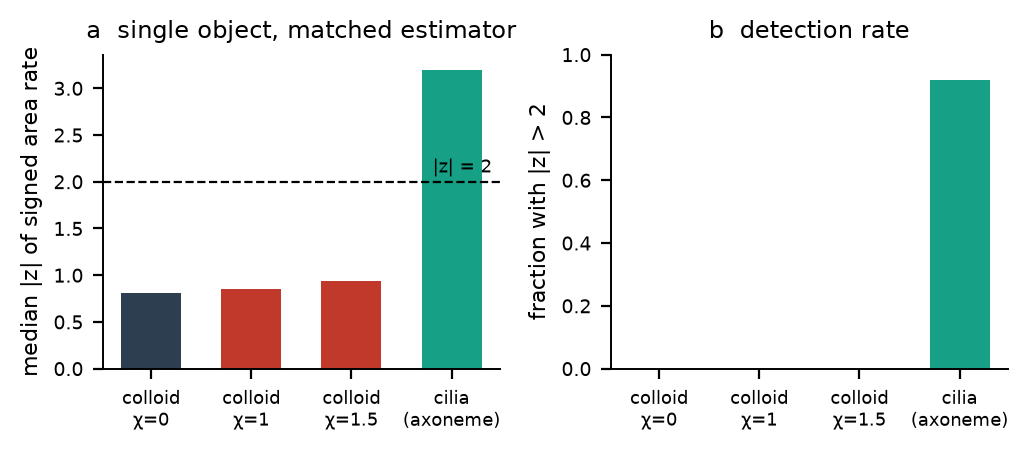
\includegraphics[width=\linewidth]{fig6_circulation.png}
\caption{\textbf{Circulation at matched level of description.} (a) Median $|z|$ of the signed area rate for a single tracked colloidal cluster at three values of $\chi$, against a single \emph{Chlamydomonas} axoneme, using the identical estimator, shape-descriptor reduction to two modes, and phase-randomised surrogate protocol. (b) The fraction of objects exceeding $|z|=2$. No circulation is detectable in the tracked colloidal clusters; axonemes show it in 92\% of cases.}
\label{fig:circulation}
\end{figure}

The colloid suspension is useful here for a reason independent of Section 3.10's inconclusive tier question: it is nonreciprocal, dissipative and strongly self-organising, and it is uncontroversially not alive. Any proposed signature of biological organisation must therefore distinguish itself from this system, not merely from equilibrium. What the comparison requires is only that the colloid be driven, far from equilibrium and demonstrably irreversible at the microscopic level, all of which Section 3.4 establishes independently.

Section 3.4 supplies the natural axis of comparison. The colloid suspension has provably positive entropy production, yet the signed area rate in every coarse observable plane is indistinguishable from the equilibrium null at both system sizes. Its irreversibility is real but microscopic: it does not survive coarse-graining.

That such circulation exists in beating axonemes is not itself new: Battle et al. \cite{r12} demonstrated probability-current loops in the phase space of beating \emph{Chlamydomonas} flagella and isolated mammalian axonemes a decade ago, establishing broken detailed balance at mesoscopic scales in active biological systems, and the subsequent literature has developed both the measurement and its coarse-graining caveats extensively \cite{r13,r14}. Our contribution here is not the observation of circulation in cilia but the \emph{controlled comparison}: the same estimator, the same surrogate protocol, and --- following the control below --- the same level of description, applied to a synthetic system whose entropy production is independently known to be positive and whose reciprocal limit is a provable equilibrium reference.

We asked whether a biological system differs on that specific axis, using published high-speed recordings of reactivated \emph{Chlamydomonas} axonemes \cite{r6,r22}: 184 usable axonemes imaged at 1000 frames per second across eight ATP concentrations from 50 to 1000 $\mu$M, 272,974 frames in total. Axoneme shapes were converted to tangent-angle representations, removing rigid translation and rotation, and reduced by principal component analysis to two dominant shape modes; the signed area rate was then computed in that plane against phase-randomised surrogates, using the identical estimator applied to the colloid observables.

We first note that the test originally planned for this dataset --- whether entropy production is quadratic in the ATP drive --- is ill-posed. The chemical potential of ATP hydrolysis depends on the concentrations of ADP and inorganic phosphate, on temperature and ionic conditions, and on standard-state corrections, none of which are reported for these reactivation buffers; it is therefore not fixed by the ATP concentration alone. What can be said without those quantities is that reactivated axonemes with an ATP-regeneration system are chemically driven far from equilibrium under all conditions in the series, so a linear-response question posed in terms of the ATP drive answers itself rather than being decided by measurement.

\begin{table}[htbp]
\caption{\emph{Chlamydomonas} axonemes by ATP concentration: beat frequency, circulation $z$-scores, and enclosed area per cycle.}
\label{tab:15}
\begin{ruledtabular}
\begin{tabular}{p{2.00cm}p{1.85cm}p{2.33cm}p{2.00cm}p{2.33cm}p{2.39cm}}
\raggedright
[ATP] $\mu$M & n & beat frequency (Hz) & median $|$z$|$ & fraction $|$z$| >$2 & $|$area per cycle$|$ \\
\hline
50 & 10 & 14.5 & 3.3 & 1.00 & 6.07 \\
66 & 15 & 23.7 & 3.3 & 1.00 & 6.24 \\
100 & 11 & 27.7 & 3.0 & 0.91 & 6.23 \\
240 & 19 & 46.3 & 2.7 & 0.89 & 6.15 \\
370 & 29 & 58.4 & 3.0 & 0.97 & 5.90 \\
500 & 13 & 91.7 & 4.5 & 0.92 & 5.95 \\
750 & 44 & 94.8 & 3.2 & 0.89 & 5.71 \\
1000 & 43 & 65.0 & 3.3 & 0.91 & 6.09 \\
\textbf{total} & \textbf{184} &  &  &  &  \\
\end{tabular}
\end{ruledtabular}
\end{table}

Pooled over all 184 axonemes, the median $|$z$|$ is 3.2, with 92\% exceeding $|$z$|$ = 2 and 55\% exceeding
$|$z$|$ = 3.

\textbf{A matched-level control.} The colloid measurement of Section 3.4 uses system-averaged network observables over $\sim$10$^{4}$ particles, whereas the cilia measurement uses the two-mode shape space of a single axoneme. These are not commensurate levels of description, and the colloid null could in principle arise from ensemble averaging alone: in an isotropic, statistically homogeneous suspension most global scalar pairs have vanishing signed area by symmetry, and phase-incoherent circulation across many clusters averages to zero --- precisely the incoherence documented in Section 3.5, where C$\sqrt{N}$ is constant.

We therefore repeated the measurement at a matched level of description: a single tracked cluster, represented by a low-order shape descriptor (deviatoric gyration tensor plus normalised third and fourth mass multipoles, the closest available analogue of the axoneme tangent-angle representation), reduced by PCA to two modes, with the identical estimator and surrogate protocol.

\begin{table}[htbp]
\caption{Circulation at a matched level of description: single tracked colloidal clusters against single axonemes.}
\label{tab:16}
\begin{ruledtabular}
\begin{tabular}{llrr}
system & level of description & median $|$z$|$ & fraction $|$z$| >$2 \\
\hline
colloid, $\chi$ = 0 & single tracked cluster & 0.81 & 0.00 \\
colloid, $\chi$ = 1 & single tracked cluster & 0.85 & 0.00 \\
colloid, $\chi$ = 1.5 & single tracked cluster & 0.94 & 0.00 \\
\emph{Chlamydomonas} axoneme & single organelle & \textbf{3.2} & \textbf{0.92} \\
\end{tabular}
\end{ruledtabular}
\end{table}

No circulation is detectable in the tracked clusters, so the contrast does not stem from the choice of coarse-graining level. Two limitations bound this. Only three to six clusters per condition persist long enough to be tracked over the 101-frame window, so the colloid side rests on few objects --- uniformly null, but few. And the persistence criterion may itself select against the signal: a cluster undergoing strong shape dynamics is less likely to survive intact for the full window, so the tracked sample may be biased toward unusually stable, non-cycling objects. The defensible claim is that circulation is absent from the clusters we could track, not that single active colloidal clusters never circulate.

\textbf{A synthetic positive control, and it changes the interpretation.} The comparison so far confounds two contrasts: biological versus synthetic, and \emph{collectively ordered} versus spatially distributed and uncoordinated. To separate them we applied the identical estimator to a Vicsek flock, which is synthetic and collectively ordered, in four variants:

\begin{table}[htbp]
\caption{Vicsek-type ensembles in four variants: polar order against circulation.}
\label{tab:17}
\begin{ruledtabular}
\begin{tabular}{lrrr}
variant & polar order & median $|$z$|$ & fraction $|$z$| >$2 \\
\hline
standard (reciprocal, no chirality) & 0.709 & 0.55 & 0.00 \\
vision cone (\textbf{nonreciprocal}, no chirality) & 0.875 & 0.32 & 0.00 \\
chiral (reciprocal, limit cycle) & 0.015 & 1.80 & 0.33 \\
chiral + vision cone & 0.069 & \textbf{5.58} & \textbf{1.00} \\
\end{tabular}
\end{ruledtabular}
\end{table}

\textbf{A purely synthetic system produces circulation stronger than the cilia signal.} Neither collective order alone nor nonreciprocity alone suffices --- both give a null --- but the chiral variants circulate strongly. Note what the polar-order column says about \emph{why}: the two chiral variants have polar order 0.015 and 0.069, an order of magnitude \emph{below} the two non-chiral ones. The strongest circulation therefore occurs where the mean heading vector is smallest. These are not strongly polar-ordered flocks, and we should not describe them as such: they are Vicsek-type ensembles with an imposed turning rate, in which the residual mean heading rotates at that rate. The control accordingly shows that circulation does not require biology; it does \emph{not} show that collective order plus chirality generates the effect.

Varying the turning rate identifies the origin: the measured area rate is 0.0056, 0.0089, 0.0141 and 0.0352 for $\omega$ = 0.005, 0.01, 0.02 and 0.04, a ratio to $\omega$ of $\approx$0.9 throughout. The signal is therefore largely the \emph{rotation of the mean heading vector at the imposed rate}, not an emergent property.

We therefore withdraw the interpretation that coarse-grained circulation distinguishes biological from non-biological organisation. What the measurement detects is whether the system possesses a \textbf{cyclic collective mode in the chosen projection} --- a structural fact about the observable, which may be emergent (the ciliary beat, arising from motor coordination) or imposed (a single-particle turning rate), and which the estimator cannot distinguish. The colloid suspension lacks such a mode at every level of description we examined; cilia possess one; and a synthetic flock can be given one by construction.

What survives is the narrower and better-supported statement: the colloid suspension has provably positive entropy production and yet no circulation in any coarse observable, at either the system-averaged or single-cluster level. Microscopic irreversibility need not project onto macroscopic observables. That is a statement about coarse-graining, not about life.

A second and unanticipated result emerges from the same analysis. The area enclosed per beat cycle is 5.71 to 6.24 in standardised shape coordinates at every ATP concentration --- flat across a twentyfold range of concentration and a sixfold range of beat frequency --- and that value is approximately 2$\pi$. We are careful about how surprising this is: if two PCA modes of a periodic waveform are standardised to unit variance and are close to phase quadrature with near-sinusoidal profiles, an enclosed area of 2$\pi$ follows almost by construction, so the value itself largely restates a property of principal component analysis applied to periodic data. The non-trivial content is the \emph{invariance} --- the tightness of the range, 5.71 to 6.24, across a twentyfold concentration range --- which says that the beat remains equally close to a clean quadrature limit cycle at every drive. On that reading the beat traces a limit cycle whose \emph{shape} is saturated and ATP-independent, while ATP sets only the \emph{rate} at which the fixed cycle is traversed, with beat frequency rising from 14.5 to approximately 95 Hz in the Michaelis--Menten manner known for axonemal dynein. Geometry and kinetics separate cleanly.

This comparison also reframes the circulation measure itself. As a probe of nonreciprocity it is poor: our strongly nonreciprocal colloid registers none. As a probe of \emph{biological} organisation it is equally poor, since an imposed turning rate reproduces and exceeds the biological signal. What it does report is whether a cyclic mode is present in the chosen projection --- a structural fact about the observable, which may be emergent or imposed, and which the estimator cannot tell apart.

We are careful about the scope of this claim. Three systems establish that the axis exists and that systems differ along it; they do not establish what governs position on it beyond the presence of a cyclic collective mode, and one synthetic system with such a mode is not a survey. Circulation measured in a two-mode projection is moreover a lower bound on irreversibility, and no system's full phase space was searched.

\subsection{A third system where the decomposition is exact: social dominance}

Every result above probes the gradient/circulating question indirectly, through the consequences of a decomposition rather than the decomposition itself. In the colloid the antisymmetric sector is something we impose; whether the resulting \emph{probability current} circulates has to be inferred from observables. There is a class of system in which the analogous decomposition can be computed exactly and in finite dimension, and it is worth doing because it tests the same proposition on data we did not generate.

For a group of n animals, the net directed interaction flow $f_{\rm ij}$ = $-$$f_{\rm ji}$ is an antisymmetric edge function on a complete graph. Filling the triangles leaves no harmonic component, so the discrete Hodge decomposition \cite{r28} is exact and strictly two-part: a gradient component that \emph{is} derivable from a scalar rank potential --- the social analogue of a conservative force --- and a curl component that is genuinely non-gradient, the rock--paper--scissors structure. The cyclic fraction $\|$curl$\|$/$\|$f$\|$ is therefore a direct measurement of the question the colloid work can only reach through consequences: \textbf{is this antisymmetric coupling a gradient, or does it circulate?}

\textbf{A methodological result comes first, because it changes what the answer is.} The decomposition must be applied to log-odds, not to raw net counts. A Bradley--Terry hierarchy has logit($p_{\rm ij}$) = $r_{i}$ $-$ $r_{j}$ exactly, so its log-odds flow is exactly a gradient, whereas the net-count flow is a \emph{logistic} function of the rank difference; a linear decomposition of counts therefore retains a cyclic component that does not vanish with more data. That component is not mathematically spurious --- it is genuinely present in the observed count-flow field --- but it is spurious \emph{as evidence of intransitivity}, which is the only thing anyone wants to read it as. On synthetic perfectly transitive groups:

\begin{table}[htbp]
\caption{Sampling floor of the Hodge cyclic fraction on synthetic perfectly transitive groups, raw counts against log-odds.}
\label{tab:18}
\begin{ruledtabular}
\begin{tabular}{rrr}
interactions per pair & cyclic fraction, raw counts & cyclic fraction, log-odds \\
\hline
5 & 0.262 $\pm$ 0.093 & 0.288 $\pm$ 0.114 \\
20 & 0.198 $\pm$ 0.054 & 0.197 $\pm$ 0.079 \\
100 & \textbf{0.157 $\pm$ 0.030} & 0.094 $\pm$ 0.042 \\
500 & \textbf{0.158 $\pm$ 0.013} & \textbf{0.044 $\pm$ 0.020} \\
\end{tabular}
\end{ruledtabular}
\end{table}

A perfectly transitive group reads as 16\% intransitive on raw counts however much data is collected. Published claims of intransitive dominance resting on a linear decomposition of counts should be checked against this floor.

\textbf{Applied to four published sociomatrices} (bundled with the \texttt{compete} package \cite{r29}), each against a null obtained by fitting that matrix's own rank potential, regenerating a perfectly transitive Bradley--Terry truth at its own per-pair counts, and re-decomposing:

\begin{table}[htbp]
\caption{Hodge decomposition of four published sociomatrices, each against a matched Bradley--Terry floor.}
\label{tab:19}
\begin{ruledtabular}
\begin{tabular}{lrrrrr}
dataset & n & interactions per ordered pair & cyclic fraction & matched transitive floor & z \\
\hline
mouse & 12 & 3.5 & 0.495 & 0.580 $\pm$ 0.054 & $-$1.6 \\
caribou & 20 & 4.3 & 0.607 & 0.579 $\pm$ 0.028 & +1.0 \\
bonobos & 6 & 49.3 & 0.341 & 0.228 $\pm$ 0.045 & +2.5 \\
people & 6 & 31.6 & 0.664 & 0.290 $\pm$ 0.074 & +5.1 \\
\end{tabular}
\end{ruledtabular}
\end{table}

The mouse hierarchy shows no excess cyclicity over a matched Bradley--Terry model --- if anything it sits 1.6$\sigma$ \emph{below} the floor, which deserves a word: a sub-floor value usually indicates the null is over-dispersed, most often because the fitted rank spacing is too compressed, so the floor itself may be mis-calibrated downward. Read the mouse result as ``no detectable excess'' rather than as positive evidence of unusual transitivity. Subject to that, it sits slightly below the floor --- so its antisymmetric social coupling is consistent with a pure gradient, with no circulating component detectable. That points the same way as the colloid result, by a route that does not depend on it --- \textbf{antisymmetry does not imply circulation} --- and in a system where the decomposition is exact rather than inferred. How much weight it can bear is limited, and the next paragraph is about that limit.

We are deliberately restrained about how much this carries. The two sparse matrices have floors near 0.58 and cannot resolve cyclicity \emph{in either direction}, so the mouse result should be read as ``consistent with transitive, with low power'' rather than as a positive finding --- and, as noted above, a value sitting below its own floor is as likely to indicate a mis-calibrated null as an unusually transitive group. The two dense matrices resolve it and disagree with each other, which establishes that the statistic has real range when the counts support it but says nothing systematic about species. All four are single unreplicated groups. The binding constraint is interaction density per ordered pair, not data availability, and the density that round-robin testing protocols produce is an order of magnitude below what the measurement needs; continuous observation of freely interacting animals is the only route we know of to close that gap.

A related observation supports the general strategy of this paper rather than any specific claim. In the longitudinal behavioural table of ref. \cite{r27}, the \emph{asymmetry} between a directed behaviour and its reverse --- chasing minus being chased, following minus being followed --- is a substantially more reproducible individual trait across days than either direction alone (intraclass correlation 0.576, 0.619, 0.719, 0.781 across four behaviour pairs, against 0.175--0.676 for the components). The per-group asymmetries also sum to zero to machine precision, which validates the rate columns internally. The antisymmetric combination being the better-behaved coordinate is exactly the premise on which the $\chi$ construction of Section 2.2 is built.

\section{Discussion}

\subsection{Isolating a sector requires a parameter that varies it alone}

The central methodological result of this work is that testing a claim about the antisymmetric sector of a coupling requires a parameter that varies that sector and nothing else, and that obtaining one is harder than it appears. Neither parameter previously proposed for the role qualifies. The coupling strength $\hat{\alpha}$ multiplies the symmetric and antisymmetric parts equally and cancels exactly from their ratio, so it tunes overall interaction strength; sweeping it produced a trend opposite to the one predicted, for reasons unrelated to reciprocity. The steric size ratio, as parameterised in the source model, varies packing while the electrohydrodynamic radii remain pinned. We note that this second failure is specific to the simulation: in experiment a particle's electrohydrodynamic and steric radii are the same physical size, so the experimental size ratio does tune nonreciprocity even though the simulated one does not.

Once a genuine knob exists, the causal claim becomes straightforward to establish and turns out to be large. Nonreciprocity drives the finite-time fragmented morphology called arrested coarsening (Section 3.2), with a same-particle reciprocal control that the source experiment cannot itself provide --- while, as Sections 3.5 and 4.5 show, simultaneously unjamming the reciprocal gel.

\subsection{The antisymmetric sector restructures rather than merely circulating}

The physical result that most changes the interpretation is that the antisymmetric sector alters equal-time structure, and does so dominantly. A description that assigns the symmetric part to energy-like structure selection and the antisymmetric part to circulation cannot be maintained: both sectors determine the structure, and here the antisymmetric one determines most of it.

This had to be so. The premise that a solenoidal coupling preserves the stationary density holds only when $\nabla \cdot$($\rho_{\rm eq}$ $\mathbf{v}$) = 0, a condition that generic nonreciprocal couplings do not satisfy. It also stands in direct tension with the source experiment, whose central finding --- that nonreciprocity arrests coarsening --- is itself a report that nonreciprocity changes steady-state structure.

Section 3.12 offers a suggestive parallel, which we are careful to label as an analogy rather than a second instance of the same proposition. In a social dominance network the antisymmetric edge flow admits an exact, finite-dimensional Hodge decomposition, and the measured flow is consistent with a pure gradient. But a Hodge curl of a static antisymmetric edge function on a complete graph of \emph{n} individuals and a probability current in a 2N-dimensional configuration space are different objects, and Section 1 lists precisely this kind of identification as one to avoid. The dominance result is therefore a structurally analogous finding in a setting where the decomposition is exact, not independent confirmation of the colloid result. Given that it is also underpowered (Section 3.12), we rest nothing on it.

What the antisymmetric sector does uniquely contribute is a positive excess dissipation, following a$\chi ^{2}$ + b$\chi$ with a resolved negative linear cross-term (Section 3.10). That form is naturally represented by a dissipation functional. We put it no more strongly than that: path actions and dissipation functions are not mutually exclusive descriptions, and the measurement does not exclude an action representation. What it does exclude is the specific claim under test --- that the antisymmetric sector merely adds a structure-preserving term to an equilibrium action. We attach no stronger claim than this: Section 3.10 also reports an apparent antisymmetric cross-coupling to a second nonreciprocal channel, which a structurally dissimilar control shows not to survive, and we do not rest any conclusion on it.

\subsection{Network observables are largely blind to nonreciprocity}

Several standard network measures fail to detect nonreciprocity here, and they fail in instructive ways.

Newman modularity is degenerate on these contact graphs. Cluster count varies by a factor of forty across the pilot-scale conditions while modularity varies by 15\%, and the two are uncorrelated; a three-cluster and a thirty-three-cluster configuration are indistinguishable. The degeneracy survives a fourfold increase in system size, so it is a property of modularity on two-dimensional contact networks at this density rather than a finite-size effect. Modularity excess over a degree-preserving null moreover \emph{decreases} with nonreciprocity and is highest in the reciprocal reference, inverting the predicted ordering.

Edge turnover fails for four independent reasons: about 70\% of its value at $\chi$ = 1 survives at $\chi$ = 0, where the probability current is provably zero; it correlates strongly with cluster morphology; its lag-one value is dominated by flicker at the contact threshold rather than by rewiring; and it becomes non-monotonic in $\chi$ at paper scale, a trend reversal that only appeared after equilibration.

The circulation measure is the most interesting failure, because it turns out to be the right instrument pointed at the wrong question. It registers nothing in the colloid suspension at either system size, yet the same estimator applied to cilia gives a median $|$z$|$ of 3.2. Circulation is therefore a poor probe of nonreciprocity. It is not, however, a probe of biological organisation either: a Vicsek-type ensemble with an imposed single-particle turning rate registers more strongly than cilia do (Section 3.11). What it detects is the presence of a cyclic mode in the chosen projection, whether that mode is emergent or imposed.

\subsection{Two kinds of arrest, distinguished by dissipation}

Section 3.5 establishes that the reciprocal reference state is a kinetically arrested gel: pair wells are 4.8 to 7.0 $k_B$T deep so bonds do not break thermally, cluster diffusion scales as 1/n so a thousand-particle cluster moves less than a particle diameter over an entire run, and --- decisively --- a condensed configuration evolved at $\chi$ = 0 with no activity whatever remains condensed. The condensate is equilibrium-accessible; the reciprocal dynamics simply cannot reach it.

This carries a caution for the wider literature on this system. Both the reciprocal control and the monodisperse reference are \emph{arrested}, and they are statistically indistinguishable from one another. ``Arrested coarsening'' therefore does not by itself indicate an actively maintained state. What distinguishes the two regimes is dissipation: exactly zero at $\chi$ = 0, positive and quadratic above it. Where an analogy to homeostatic or biological organisation is intended, the transferable quantity is an irreversibility measure rather than a structural one, since a frozen aggregate and a dynamically maintained one may be structurally similar while differing absolutely in dissipation.

\subsection{Arrest without a steady state}

The finite-cluster state of this model is real, reproducible and long-lived --- it is what one observes on the timescale of the source experiment --- but it is not asymptotic. Continued to twice the source duration, the same system phase-separates. A variational account that attributes the finite-cluster state to a steady-state balance between energy and connection cost is therefore describing a transient rather than an attractor.

The transient is nonetheless long, and quantifiably so. Fitting the largest cluster as $S$ $\sim$ A $t^{z}$ gives z between 0.27 and 0.42 for every nonreciprocal condition. \emph{If} that growth law, its amplitude and its mechanism persist up to system-spanning scales, the crossover time scales as N\textasciicircum\{\}(1/z) with 1/z between 2.4 and 3.7, and a tenfold larger system would remain in the finite-cluster regime between 250 and 5000 times longer. We stress that this is an extrapolation under the observed growth law, not a measured lifetime scaling: our largest system spans a factor of four in $N$, and nothing here verifies that a single power law survives to macroscopic sizes. Read with that caveat, it suggests that in a macroscopic suspension the distinction between long-lived transient and steady state may be difficult to draw operationally. This reconciles our result with the source report, which is accurate for its own system size and duration.

A related inversion deserves explicit statement, because the phrase ``arrested coarsening'' invites the opposite reading. The reciprocal case has by far the \emph{slowest} coarsening (z = 0.089), and every nonreciprocal case sits near the diffusion-limited value of 1/3. Nonreciprocity accelerates growth of the majority phase --- it unjams the gel --- while sustaining a population of small fragments. ``Arrest'' in this model therefore denotes a persistent fragment population, not a slowed majority phase, and the genuinely arrested state is the reciprocal one.

\subsection{What the biological comparison does and does not establish}

The colloid suspension is nonreciprocal, dissipative and strongly self-organising, and it is uncontroversially not alive. That alone makes it a useful control, and the comparison below does not depend on the tier question of Section 3.10 --- which, as reported there, our measurements leave undetermined. What the comparison requires is only that the colloid be driven, far from equilibrium, and demonstrably irreversible at the microscopic level, all of which is established independently in Section 3.4.

Cilia differ from the colloid on a measurable axis --- their irreversibility survives coarse-graining --- and it is tempting to read that as a signature of biological organisation. A synthetic control shows that it is not. A chiral Vicsek-type ensemble, given a turning rate by construction, circulates more strongly than cilia do, while a nonreciprocal but non-chiral variant circulates not at all despite far higher polar order. The discriminating property is therefore the presence of a cyclic mode in the projection, not biology and not nonreciprocity.

We regard this as the more useful outcome. It converts a claim we could not have defended into a narrower one that the data support: microscopic irreversibility need not project onto macroscopic observables, and whether it does is a structural property of the system's collective modes rather than of its provenance. It also identifies what a genuine biological signature would have to do --- distinguish an emergent limit cycle, such as the coordinated ciliary beat, from an imposed one, such as a single-particle turning rate --- which the area-rate estimator by construction cannot.

\subsection{Consequences for a network-weighted action principle, and for minimum-action learning}

One specific formulation of the decomposition tested above is the Network-Weighted Action Principle (NWAP) \cite{r9,r33}, which posits that a system minimises

\begin{equation}
S_{\rm NW}=\int (E-I+A\cdot C)\,dt
\end{equation}

with E an energetic or operational cost, I the system's information or diversity, A a connectivity weight and $C$ the cost of forming and maintaining connections. It has been applied to physiological causation \cite{r9}, symbolic law discovery \cite{r31}, neural architecture \cite{r32}, and marine metabolic networks \cite{r30}. What this study tests is a \emph{directed-graph extension} of it --- unpublished, and formulated by the present author while designing this study --- that makes the symmetric/antisymmetric assignment explicit, together with one published prediction, the modularity-excess signature of ref. \cite{r30}.

\emph{That framework is the present author's own, and this study was undertaken to test its predictions; we state the outcome directly and note the conflict of interest.} The outcome is mixed, and the parts that fail and the parts that survive are informative in different ways.

\textbf{The decomposition proved experimentally useful.} The directed-graph extension holds that a nonreciprocal coupling should be split into symmetric and antisymmetric sectors, with the antisymmetric sector carrying the nonequilibrium content. Constructing that split is what made every subsequent measurement possible, and the prediction that cluster statistics are controlled by the antisymmetric-to-symmetric ratio is borne out across two system sizes, with a same-particle reciprocal control the source experiment cannot itself provide. We are deliberate about what this does and does not establish. The decomposition is an algebraic operation, and showing that cluster statistics depend strongly on $\chi$ demonstrates that the antisymmetric sector matters. It does not validate the NWAP functional, its information term, its connection-cost term, or any predicted functional relationship between them. The useful thing that survives is the instrument, not the theory behind it.

We state this more carefully than a rank correlation would suggest. The Spearman coefficient across the $\chi$ sweep is $\rho$ = +0.931, but the underlying relation is \emph{not monotonic}: cluster count dips to 2.2 at $\chi$ = 0.25, a factor of five below its reciprocal value, before rising by two orders of magnitude (Section 3.5). A rank correlation is a poor summary of such a curve. The defensible statement is that nonreciprocity strongly controls cluster statistics, that the control is non-monotonic, and that no proposed functional form --- NWAP's included --- predicts the dip. This is, to our knowledge, the first NWAP prediction tested in a controlled physical system rather than by meta-analysis, and on this point it succeeds.

\textbf{The mechanism attributed to that sector does not survive.} Three specific claims fail:

\emph{Solenoidality.} The premise that the antisymmetric sector cannot alter a static structural observable is contradicted directly: cluster count, a single-snapshot quantity, changes by a factor of 12.4 when the antisymmetric coupling alone is scaled. The premise holds only where $\nabla \cdot$($\rho_{\rm eq}$ $\mathbf{v}$) = 0, which generic nonreciprocal couplings do not satisfy. It is also in tension with the source experiment, whose central result --- nonreciprocity arrests coarsening --- is itself a statement that nonreciprocity changes steady-state structure.

\emph{Circulation.} No circulation is detectable in any coarse network observable, at either system size, against a provable equilibrium null. The ``circulating partition'' half of the prediction has no empirical support in this system, notwithstanding that the system is genuinely irreversible.

\emph{The modularity signature.} This is the one prediction with a published pedigree. Ref. \cite{r30} establishes, in marine metabolic networks, that modularity \emph{excess} over a null --- rather than absolute modularity, which there arises from sparsity alone --- is the informative signature of constrained organisation, reporting $\Delta$Q $\approx$ 0.15--0.40 over configuration-model, label-permutation and bipartite-incidence nulls. Carried over to the present system, the directed-graph extension predicts a sustained excess in the nonreciprocal case relative to a reciprocal null. \textbf{It fails with inverted sign.} Our excess over a degree-preserving (configuration-model) null is of comparable magnitude to theirs, 0.38--0.46, so the quantity is not simply absent; but it \emph{decreases} monotonically with nonreciprocity and is largest in the reciprocal reference. The underlying reason is that Newman modularity is degenerate on these contact graphs --- cluster count varies forty-fold while $Q$ varies by 15\%, and the two are uncorrelated --- so the test could not have discriminated in either direction. We note that this diagnosis is specific to two-dimensional contact networks at this density and does not transfer to the sparse bipartite metabolic networks of ref. \cite{r30}, where the excess is measured against a different null on a different topology.

\textbf{What the antisymmetric sector actually contributes is dissipation.} Section 3.10 establishes that it produces a positive entropy production, quadratic in the coupling at fixed structure. A positive quadratic in the drive is the functional form of a dissipation functional, not of an action extremum. We had also reported an antisymmetric, hence non-dissipative, cross-coupling to a second nonreciprocal channel; that result did not survive its control and is withdrawn, so the claim here rests on the dissipation alone.

\textbf{Where this leaves the framework.} We would draw three conclusions, offered constructively.

First, the broadening that NWAP requires is not ad hoc. There is a standard hierarchy of variational principles for stochastic dynamics, and least action does not in fact fail for nonreciprocal systems: the Onsager--Machlup action is well defined for any drift field. What fails is the equilibrium corollary. NWAP's Triple-Action, with its explicit information term traded against an energy term under structural constraints, has the formal shape of a Maximum Caliber functional \cite{r10} --- the path-entropy principle that reduces to MaxEnt statically and to Onsager near equilibrium. Placing NWAP as a constrained member of that family, with network-structural rather than thermodynamic constraints, would give it a principled home and two checkable reductions: it should reduce to a Rayleighian at weak drive and to free-energy minimisation at zero drive.

This also sharpens NWAP's relation to its neighbours. It has been positioned alongside the free-energy principle \cite{r34} and dissipative adaptation \cite{r35}, both of which are likewise functional-minimisation accounts of organisation. The distinction our results suggest is not which functional is minimised but \emph{what the functional is allowed to govern}: on the evidence here, a variational account of this kind can describe the dynamics at fixed structure, and the transition that selects the structure is a separate problem. That boundary applies to the neighbouring frameworks as much as to NWAP, and is a more useful place to look for discriminating tests than the choice of functional.

Second, the discipline that keeps such a broadening falsifiable is that each tier carries its own experimental signature and membership must be \emph{measured}. We tested three such signatures here. A framework asserting that ``some variational principle applies'' forbids nothing; one asserting tier-II membership predicts quadratic dissipation, Onsager reciprocity, and a single effective temperature, each of which can fail independently. In this system none of the three returns a decisive positive: the first is near-tautological at fixed structure, the second does not survive a structurally dissimilar control, and the third is not a well-defined quantity. That is a harder outcome to accommodate than a clean pass or a clean fail, and it is one that no amount of reinterpretation could have produced from the framework alone. It also suggests that the tier taxonomy, useful as a way of organising what to measure, is not straightforwardly decidable by measurement in a system like this one.

Third, the boundary of applicability should be stated rather than obscured. Entropy production here is quadratic \emph{at fixed structure}, while the structural response to the antisymmetric coupling is strongly non-linear. Whatever variational description turns out to apply --- and Section 3.10 does not establish that a Rayleighian does --- its scope can extend at most to the dynamics at fixed structure. Structure selection is not explained by the equilibrium-like or Rayleighian constructions tested here. We put it that way rather than claiming no variational principle covers it: nonequilibrium quasipotentials, large-deviation theory, macroscopic fluctuation theory and model-specific constructions all address aspects of structure selection, and we have not tested them. Since structure selection is precisely what NWAP was built to explain, this identifies the gap that new theory would have to fill, and it is a more useful result for the framework than a claim of coverage would have been.

\textbf{Connection to minimum-action learning.} The same programme has a computational arm, Minimum-Action Learning \cite{r31}, whose discriminating criterion is energy conservation under dynamical rollout. That criterion presupposes a conserved energy, which exists precisely when the force is reciprocal --- exactly at $\chi$ = 0 here, and nowhere above it. The method should therefore succeed at $\chi$ = 0 and degrade as $\chi$ grows, with the conservation residual it computes being, up to normalisation, the dissipation measured in Section 3.10. Replacing energy conservation with a dissipation-consistency criterion would be the natural extension, and the trajectories generated here are a ready benchmark for it. We test none of this and note it only as an implication.

\textbf{A note on the empirical hook.} The reanalysis originally proposed to connect NWAP to this literature --- computing modularity excess on published trajectory data --- should not be attempted; we ran it and it fails with inverted sign for reasons intrinsic to the measure. The analysis that does work, and that we would suggest in its place, is the $\chi$ decomposition with cluster statistics and entropy production as the observables, together with the two-kinds-of-arrest distinction of Section 4.4 as the bridge to the biological claim.

\section{Limitations}

\textbf{The reciprocity parameter is synthetic.} $\chi$ is a control parameter of our construction rather than an experimental one, and $\chi$ $>$ 1 lies outside the derived electrohydrodynamic model. Values above unity are reported as trend evidence only. The corresponding physical knob is the electrohydrodynamic radius contrast, which is experimentally accessible but which we did not sweep because it confounds the nonreciprocity ratio with the overall coupling strength of the small--small pair interaction.

\textbf{Entropy production rests on a subtracted artifact.} The Stratonovich heat estimator subtracts two nearly cancelling terms of order $\mu |$F$| ^{2}$, and its discretisation residual exceeds the signal at the production timestep. It is usable only at much smaller timestep with a paired same-configuration control, and it resolves only for $\chi$ $\gtrsim$ 0.75. The bias probe is a single stochastic realisation and failed on one of three configurations in the pilot measurement.

\textbf{No tier-II signature was established.} Of the three near-equilibrium diagnostics tested in Section 3.10, one is near-tautological at fixed structure, one does not survive a structurally-dissimilar control, and one is not a well-defined quantity out of equilibrium. We therefore make no claim about which variational tier this system occupies, and readers should not infer one from the positive entropy production alone.

\textbf{Response coefficients required a plateau test.} Both the Onsager and effective-temperature measurements produced stable, small-error-bar values under protocols that were subsequently shown to be wrong, and in each case only a scan against the measurement window or the perturbation strength revealed the problem. We therefore report no response coefficient that has not been shown to plateau. Readers should treat any such coefficient reported without that check, in this literature generally, with corresponding caution.

\textbf{The analysis graph is undirected.} Contact graphs are constructed with \texttt{nx.Graph} throughout, so the directed-graph content of the motivating proposal is untested by this pipeline. Building the directed contact graph --- with edges signed by the nonreciprocal force imbalance --- remains the natural next step for that specific claim.

\textbf{Box geometry in the source-specification replicate.} The source domain is 648 $\times$ 360 $\mu$m, an aspect ratio of 1.8, whereas the replicate uses an equal-area square. We tested this directly with a rectangular-box integrator (\texttt{simulate\_rect.py}, validated as bitwise identical to the square kernel in the $L_x$ = $L_y$ limit): at $N$ = 4000, $\chi$ = 1.5, matched area, density and duration, the 1.8:1 rectangle gives lcf = 0.804 $\pm$ 0.008 against 0.779 $\pm$ 0.004 for the square, a difference of 3\%. The square approximation is therefore justified at this system size, though we have not repeated the test at $N$ = 22,000.

\textbf{$\sigma^2_v$ is not comparable to the source definition.} The source reports 5 $\times$ 10$^{-3}$ and 2 $\times$ 10$^{-2}$ $\mu m^{2}$/$s^{2}$ for monodisperse and bidisperse respectively, a ratio of 4; ours is approximately 90. Ours is the variance of \emph{speed} coarse-grained over one snapshot interval rather than an instantaneous velocity variance, so the discrepancy is most likely definitional, but this cannot be confirmed without the source sampling interval.

\textbf{Pairwise forces only.} Many-body hydrodynamics are absent, inherited from the source model, which shifts absolute cluster sizes and may bear directly on the transience result of Section 3.8: hydrodynamic interactions are exactly the class of ingredient that could stabilise finite clusters indefinitely.

\textbf{The $\chi$ = 0 entropy production is zero by construction, not by measurement.} The paired protocol subtracts each configuration's own $\chi$ = 0 bias probe, so at $\chi$ = 0 the estimate and its control are the same quantity and the net is identically zero. The $\chi$ = 0 row therefore validates nothing; the argument that $\chi$ = 0 has zero current is the analytic one of Section 2.3, not an empirical one. What the paired protocol does establish is that the \emph{excess} over that reference is resolved for $\chi$ $\gtrsim$ 0.75.

\textbf{The dominance analysis is underpowered where it matters most.} Of the four published matrices in Section 3.12, the two built by round-robin testing have 3.5 and 4.3 interactions per ordered pair against a matched transitive floor near 0.58, so they cannot resolve cyclicity in either direction. The rodent result is therefore ``consistent with a gradient, with low power'' and not a positive finding. All four are single unreplicated groups, and the floor is computed under a Bradley--Terry null; a different transitive generative model would shift it.

\textbf{Sample sizes in the biological comparison.} The cilia analysis uses two shape modes and phase-randomised surrogates; a stricter surrogate (iterative amplitude-adjusted Fourier transform), which preserves the amplitude distribution as well as the power spectrum, would make the null more conservative and would likely reduce the reported z-scores. Beat frequency is a spectral-peak estimate and is not monotonic at the top of the ATP range.

\subsection{Pre-registration against outcome}

Thresholds for the $\chi$ experiment were committed in \texttt{EXPERIMENT.md} before any $\chi$ run was executed. Three claims have since been withdrawn across revisions, so it is worth setting the pre-registered predictions against what happened. Two of the four pre-registered hypotheses failed, and one of the failures killed the study's original headline.

\begin{table}[htbp]
\caption{Pre-registered predictions against outcomes. Thresholds were committed in \texttt{EXPERIMENT.md} before any $\chi$ run.}
\label{tab:20}
\begin{ruledtabular}
\begin{tabular}{p{1.00cm}p{3.26cm}p{2.74cm}p{7.27cm}}
\raggedright
\# & pre-registered prediction & pre-committed threshold & outcome \\
\hline
H1 & edge turnover increases monotonically in $\chi$ & Spearman $\rho$ $>$ 0, p $<$ 0.01 & \textbf{passed at pilot scale, failed at paper scale.} Turnover is non-monotonic in $\chi$, peaking at $\chi$ = 0.75 (\S{}3.7). The monotonicity was an artifact of not having reached steady state. \\
H2 & structure moves far less than currents (``frozen $Q$, circulating partition'') & $R_{Q}$ $<$ 0.1 \textbf{and} $R_{\rm turnover}$ $>$ 0.5 & \textbf{failed as intended, and informatively.} $Q$ did stay within threshold, but not because structure is preserved: $n_{\rm cl}$ moves by 12.4$\times$ (\S{}3.2) and $Q$ is degenerate on these graphs (\S{}3.3). The pre-committed reading ``turnover rises, $Q$ flat $\Rightarrow$ prediction confirmed'' would have been wrong, which is why \S{}3.3 tests Q's discriminating power directly. \\
H3 & $\sigma^2_v$ increases with $\chi$ & directional & \textbf{passed.} $\rho$ = +0.975, p = 7$\times$10$^{-12}$ (\S{}3.2). \\
H4 & at $\chi$ = 0 turnover falls toward the monodisperse baseline & if not, mono/bi gap was polydispersity & \textbf{partial, and the informative arm.} Turnover at $\chi$ = 0 is 0.260 against 0.148 monodisperse and 0.378 at $\chi$ = 1, so about half the gap is polydispersity (\S{}3.6). The pre-committed reading --- that this ``falsifies the project's headline interpretation while leaving the measurement intact'' --- is what happened, and is why edge turnover is retired as a probe in \S{}3.7. \\
\end{tabular}
\end{ruledtabular}
\end{table}

Two points about this table. First, the one hypothesis that passed cleanly (H3) is the one whose observable, $\sigma^2_v$, survived scrutiny; the two that failed are the ones built on edge turnover and modularity, both of which \S{}3.7 and \S{}3.3 go on to disqualify. Second, the pre-committed failure readings were followed rather than reinterpreted: H4's stated consequence was that the headline interpretation dies, and it did. The withdrawals documented throughout this paper are the pre-registration working as intended, not evidence against the design.

\section{Conclusions}

\begin{enumerate}
\item Isolating the antisymmetric sector of a nonreciprocal coupling requires a parameter that varies it alone. Neither the coupling strength nor the steric size ratio does so; the reciprocity mixing parameter $\chi$ does. At $\chi$ = 0 the \emph{dynamics} are equilibrium-compatible --- conservative forces with a uniform fluctuation--dissipation ratio, hence detailed balance and zero stationary current --- which is a stronger reference than a control, though the finite-time configurations it realises are kinetically trapped and do not sample the corresponding Boltzmann distribution.
\item Nonreciprocity produces the finite-time fragmented morphology conventionally called arrested coarsening, in the operational sense defined in Section 3.2 --- many coexisting, continuously reorganising clusters --- while simultaneously unjamming the reciprocal gel. At $N$ = 4000 the cluster count rises by a factor of 12.4 from $\chi$ = 0 to $\chi$ = 1.5 with the reciprocal coupling held bit-for-bit fixed; the pilot scale gives 9.8$\times$ for the same contrast, so the effect is reproduced at a second system size but the factor itself is the $N$ = 4000 number.
\item The antisymmetric sector alters \emph{static} structure and is not structure-preserving. The solenoidal premise fails, and would have had to, since it contradicts the source experiment's own central finding.
\item Newman modularity is degenerate on these networks and its excess over a degree-preserving null runs opposite to the predicted direction. Cluster-size statistics, not modularity, carry the signature.
\item No circulation is detectable in the coarse network observables examined, yet the excess dissipation over the reciprocal control is positive and resolved for $\chi$ $\gtrsim$ 0.75. Across the whole drive range it follows EPR = a$\chi ^{2}$ + b$\chi$ with b $<$ 0, the negative linear cross-term being resolved at 5.6$\sigma$ at low drive. The dynamics are genuinely irreversible; that irreversibility did not appear in any projection we examined, which is a statement about those projections rather than about the dynamics.
\item The reciprocal reference state is a kinetically arrested gel, not an equilibrium structure. Weak nonreciprocity unjams it, producing a non-monotonic dependence of cluster count on $\chi$, and the genuinely arrested state is the reciprocal one.
\item No finite characteristic cluster size is selected: the largest cluster grows as $N^{1.00\pm0.07}$ across a fourfold range of system size, and the largest-cluster fraction is flat (0.79, range 0.71--0.86) across that range without any fit. The scale that is selected, at approximately seven to eight particles, is an \textbf{event-rate crossover} --- the size at which per-cluster splitting gives way to merging --- rather than a stable organisational level. We stop short of calling it a critical nucleus, which would require the size drift $\langle \Delta S|S\rangle$ to change sign there or a committor of one half, neither of which we measured. The finite-cluster state is a long-lived transient; \emph{if} the observed growth law persists to system-spanning scales, its crossover time would scale as N\textasciicircum\{\}(1/z) with 1/z between 2.4 and 3.7, but that is an extrapolation from a fourfold range of $N$ and not a measured lifetime scaling.
\item \textbf{Variational tier membership is undetermined by the three diagnostics we tested, and none of them returns a decisive positive.} Entropy production is quadratic to within 4.8\% over a fifteenfold range of signal, but at fixed structure that form is close to guaranteed by the construction of $\chi$, so the measurement is best read as a validation of the entropy-production estimator. A differential cross-response between two nonreciprocal channels is predominantly antisymmetric when the channels share a structure, but a structurally dissimilar control inverts the pattern, so we withdraw the reciprocity reading. The third returns a definite negative: the fluctuation--dissipation ratio grows as $t^{0.89}$ across a fourfold window (5.2 $\rightarrow$ 9.5 $\rightarrow$ 17.7 $k_BT$) while calibrating to unity at equilibrium, so no effective temperature exists on this coordinate. About half that growth is translation of the whole aggregate under a net internal force; the rest survives a control that removes it. Whatever variational description applies, its scope is at most the dynamics at fixed structure, since structure selection itself remains uncovered.
\item The difficulty in conclusion 8 is itself part of the finding: of three commonly invoked near-equilibrium signatures, two are defeated by their own construction rather than by the physics --- one near-tautological given how $\chi$ is built, one an artifact of giving two response channels the same structure. Tier taxonomies are useful for deciding what to measure and harder than they appear to decide by measurement. Chasing the third turned up a mechanism rather than a result: nonreciprocal forces do not sum to zero, so the centre of mass drifts, near-ballistically over short windows ($t^{1.96}$ against $t^{1.01}$ at $\chi$ = 0). That drift is finite-size --- amplitude falling roughly as $N^{-1/2}$ --- and decorrelates over long runs, so we report it as a bounded observation and not as a new phenomenon. The colloid suspension none the less serves as a control for systems that are driven but not alive, which requires only that it be far from equilibrium and demonstrably irreversible --- both established independently.
\item For the Network-Weighted Action Principle specifically, the structural proposal survives and its quantitative prediction is borne out though non-monotonically, while the mechanism attributed to the antisymmetric sector --- solenoidality, circulation, and a modularity signature --- fails on all three counts. The sector's measurable contribution is a positive excess dissipation, following a$\chi ^{2}$ + b$\chi$ with b $<$ 0. That form is naturally represented by a dissipation functional; it does not support the stronger claim that the antisymmetric sector merely adds a structure-preserving term to an equilibrium action.
\item In published social-dominance matrices, where the symmetric/antisymmetric decomposition is exact and finite-dimensional rather than inferred, the measured antisymmetric coupling is consistent with a pure gradient and shows no detectable circulating component --- though at an interaction density per ordered pair where the measurement has limited power, so this is ``consistent with a gradient'', not a demonstration of one. It none the less points the same way as the colloid result, by an independent route: antisymmetry does not imply circulation. Separately, the Hodge decomposition of dominance must be computed on log-odds: on raw counts a perfectly transitive group reads as 16\% intransitive however much data is collected, which is a floor that published intransitivity claims should be checked against.
\item Cilia show macroscopic circulation in shape space where the colloid, at both system-averaged and single-cluster level, shows none. A synthetic chiral flock, however, circulates more strongly than cilia while a nonreciprocal non-chiral flock shows none at all, so the measured property is the presence of a cyclic collective mode rather than biological organisation. The defensible conclusion is that microscopic irreversibility need not project onto macroscopic observables, and that whether it does is a structural property of the system's collective modes.
\end{enumerate}

\section{Data and code availability}

All code, per-run summaries and figures are in the repository. Simulation: \texttt{simulate.py} (model, reciprocity parameter, sweeps), \texttt{simulate\_par.py} (thread-parallel force kernel, validated to 8.9 $\times$ 10$^{-15}$ against the serial kernel), \texttt{simulate\_rect.py} (rectangular box, bitwise identical to the square kernel at $L_x$ = $L_y$), \texttt{continue\_run.py} (run continuation). Analysis: \texttt{analyze.py} (network observables), \texttt{epr\_probe.py} (entropy production), \texttt{onsager.py}, \texttt{onsager\_equil.py} and \texttt{onsager\_equil2.py} (cross-response), \texttt{fdt.py} (effective temperature), \texttt{arrest\_test.py} (configuration-swap test), \texttt{crossover.py} (per-cluster propulsive force), \texttt{irreversibility.py} and \texttt{benchmark\_irrev.py} (time-series estimators and their calibration against an exactly solvable biased ring walk). Comparison systems: \texttt{cilia\_analysis.py}, \texttt{single\_cluster\_circulation.py}, \texttt{vicsek.py}, \texttt{hodge\_dominance.py}, \texttt{forkosh\_asymmetry.py}. Controls added in revision: \texttt{drift\_control.py} (whether the collective-coordinate superdiffusion is whole-system drift) and \texttt{fdt\_driftfree.py} (effective temperature with and without that drift, from the same starts). Figures: \texttt{make\_figures.py}. Validation: \texttt{tests/test\_reciprocity.py} (the $\chi$ construction).

Supplementary figures, not reproduced here: \texttt{modularity\_test.png} (baseline four-panel), \texttt{snapshots.png} (final-frame renders), \texttt{coarsening.png} (trajectories by $\chi$), \texttt{chi\_test.png}, and \texttt{sweep.png} (the two mis-specified sweeps, retained for the record).

Supporting documents: \texttt{AUDIT.md} (observable validity), \texttt{EXPERIMENT.md} (pre-registered protocol with thresholds committed before running), \texttt{BOX\_SCALING.md}, \texttt{COARSENING.md}, \texttt{ONSAGER\_RESULT.md}, \texttt{CILIA\_RESULT.md}, \texttt{DOMINANCE\_HODGE\_RESULT.md}, \texttt{FORKOSH\_RESULT.md}, \texttt{VARIATIONAL\_FAMILY.md}, \texttt{FOLLOWUP.md}, \texttt{TODO.md}.

Raw trajectories (approximately 4 GB) are not version-controlled. The cilia dataset is openly available from Dryad under CC0 \cite{r6}.

\begin{thebibliography}{99}
\bibitem{r1} S. Hara, M. Okada, K. Kittaka, $S$. Tanami, Y. Iwasaki, H. Ishikawa, K. Yoshii, Y. Sumino. \emph{Arrested coarsening in active colloidal suspensions driven by nonreciprocal electrohydrodynamic interactions.} Phys. Rev. Lett. \textbf{137}, 068302 (2026). DOI 10.1103/96ky-d1p9; arXiv:2509.23164.
\bibitem{r2} M. Fruchart, $R$. Hanai, P. B. Littlewood, V. Vitelli. \emph{Non-reciprocal phase transitions.} Nature \textbf{592}, 363 (2021).
\bibitem{r3} M. E. J. Newman. \emph{Modularity and community structure in networks.} PNAS \textbf{103}, 8577 (2006).
\bibitem{r4} S. Fortunato, M. Barth\'elemy. \emph{Resolution limit in community detection.} PNAS \textbf{104}, 36 (2007).
\bibitem{r5} K. Sekimoto. \emph{Stochastic Energetics.} Lecture Notes in Physics 799, Springer (2010).
\bibitem{r6} V. F. Geyer, J. Howard, P. Sartori. \emph{Ciliary beating patterns map onto a low-dimensional behavioural space.} Nature Physics \textbf{18}, 1465 (2022), DOI 10.1038/s41567-021-01446-2. Dataset: Dryad, DOI 10.5061/dryad.0gb5mkm2j.
\bibitem{r7} L. Onsager. \emph{Reciprocal relations in irreversible processes.} Phys. Rev. \textbf{37}, 405 (1931).
\bibitem{r8} H. B. G. Casimir. \emph{On Onsager's principle of microscopic reversibility.} Rev. Mod. Phys. \textbf{17}, 343 (1945).
\bibitem{r9} M. G. Frasch. \emph{Causal thinking in physiology: a search for vertically organising principles.} The Journal of Physiology (2026), DOI 10.1113/JP290762. \emph{(Defines the Network-Weighted Action Principle, $S_{\rm NW}$ = $\int$(E $-$ I + A$\cdot$C) dt. Author's own prior work; see the disclosure in Section 4.7.)}
\bibitem{r10} E. $T$. Jaynes. \emph{Macroscopic prediction}, in Complex Systems --- Operational Approaches, Springer (1985), for Maximum Caliber; see also P. $D$. Dixit et al., J. Chem. Phys. \textbf{148}, 010901 (2018).
\bibitem{r11} L. F. Cugliandolo. \emph{The effective temperature.} J. Phys. A \textbf{44}, 483001 (2011).
\bibitem{r12} C. Battle, $C$. P. Broedersz, $N$. Fakhri, V. F. Geyer, J. Howard, $C$. F. Schmidt, F. $C$. MacKintosh. \emph{Broken detailed balance at mesoscopic scales in active biological systems.} Science \textbf{352}, 604 (2016).
\bibitem{r13} F. $S$. Gnesotto, F. Mura, J. Gladrow, $C$. P. Broedersz. \emph{Broken detailed balance and non-equilibrium dynamics in living systems: a review.} Rep. Prog. Phys. \textbf{81}, 066601 (2018).
\bibitem{r14} J. Gladrow, $C$. P. Broedersz, $C$. F. Schmidt. \emph{Nonequilibrium dynamics of probe filaments in actin--myosin networks.} Phys. Rev. E \textbf{96}, 022408 (2017).
\bibitem{r15} A. V. Ivlev, J. Bartnick, M. Heinen, $C$.-R. Du, V. Nosenko, H. L\"owen. \emph{Statistical mechanics where Newton's third law is broken.} Phys. Rev. $X$ \textbf{5}, 011035 (2015).
\bibitem{r16} S. Saha, J. Agudo-Canalejo, $R$. Golestanian. \emph{Scalar active mixtures: the non-reciprocal Cahn--Hilliard model.} Phys. Rev. $X$ \textbf{10}, 041009 (2020).
\bibitem{r17} Z. You, A. Baskaran, M. $C$. Marchetti. \emph{Nonreciprocity as a generic route to traveling states.} PNAS \textbf{117}, 19767 (2020).
\bibitem{r18} S. A. M. Loos, $S$. H. $L$. Klapp. \emph{Irreversibility, heat and information flows induced by non-reciprocal interactions.} New J. Phys. \textbf{22}, 123051 (2020).
\bibitem{r19} \'E. Fodor, $C$. Nardini, M. E. Cates, J. Tailleur, P. Visco, F. van Wijland. \emph{How far from equilibrium is active matter?} Phys. Rev. Lett. \textbf{117}, 038103 (2016).
\bibitem{r20} C. Nardini, \'E. Fodor, E. Tjhung, F. van Wijland, J. Tailleur, M. E. Cates. \emph{Entropy production in field theories without time-reversal symmetry.} Phys. Rev. $X$ \textbf{7}, 021007 (2017).
\bibitem{r21} M. Doi. \emph{Onsager's variational principle in soft matter.} J. Phys.: Condens. Matter \textbf{23}, 284118 (2011).
\bibitem{r22} P. Sartori, V. F. Geyer, A. Scholich, F. J\"ulicher, J. Howard. \emph{Dynamic curvature regulation accounts for the symmetric and asymmetric beats of Chlamydomonas flagella.} eLife \textbf{5}, e13258 (2016).
\bibitem{r23} B. H. Good, Y.-A. de Montjoye, A. Clauset. \emph{Performance of modularity maximization in practical contexts.} Phys. Rev. E \textbf{81}, 046106 (2010).
\bibitem{r24} T. P. Peixoto. \emph{Descriptive vs. inferential community detection in networks.} Cambridge University Press (2023).
\bibitem{r25} R. Kubo. \emph{The fluctuation-dissipation theorem.} Rep. Prog. Phys. \textbf{29}, 255 (1966).
\bibitem{r26} U. Seifert. \emph{Stochastic thermodynamics, fluctuation theorems and molecular machines.} Rep. Prog. Phys. \textbf{75}, 126001 (2012).
\bibitem{r27} O. Forkosh, $S$. Karamihalev, $S$. Roeh, et al., A. Chen. \emph{Identity domains capture individual differences from across the behavioral repertoire.} Nature Neuroscience \textbf{22}, 2023 (2019). Data: github.com/OrenForkosh/IdentityDomains (MIT licence).
\bibitem{r28} X. Jiang, $L$.-H. Lim, Y. Yao, Y. Ye. \emph{Statistical ranking and combinatorial Hodge theory.} Mathematical Programming \textbf{127}, 203 (2011).
\bibitem{r29} J. P. Curley. \emph{compete: analyzing competitive interaction data.} $R$ package (2016), github.com/jalapic/compete.
\bibitem{r30} M. G. Frasch. \emph{Modularity emerges from action-functional constraints in marine metabolic networks: a biology-scale validation of the Network-Weighted Action Principle.} arXiv:2605.05254 (2026). \emph{(Author's own prior work: the source of the modularity-excess prediction tested in Sections 3.3 and 4.7.)}
\bibitem{r31} M. G. Frasch. \emph{Minimum-Action Learning: energy-constrained symbolic model selection for physical law identification from noisy data.} arXiv:2603.16951 (2026). \emph{(Author's own prior work.)}
\bibitem{r32} M. G. Frasch. \emph{minAction.net: energy-first neural architecture design --- from biological principles to systematic validation.} arXiv:2604.24805 (2026). \emph{(Author's own prior work.)}
\bibitem{r33} M. G. Frasch. \emph{Bridging mathematical formalism and physical law: a network-weighted action framework for foundation model training.} HAL preprint hal-05347658 (2025). \emph{(Author's own prior work.)}
\bibitem{r34} K. Friston. \emph{The free-energy principle: a unified brain theory?} Nature Reviews Neuroscience \textbf{11}, 127 (2010).
\bibitem{r35} J. $L$. England. \emph{Statistical physics of self-replication.} J. Chem. Phys. \textbf{139}, 121923 (2013).
\end{thebibliography}

\end{document}
